\documentclass[FM,BP]{tulthesis}
% tento dokument používá balíky specifické pro XeLaTeX a lze jej přeložit
% jen XeLaTeXem, nemáte-li instalována použitá (komerční) písma, změňte
% nebo vymažte příkazy \set...font na následujících řádcích
\newcommand{\verze}{1.10}

\usepackage{polyglossia}
\setdefaultlanguage{czech}
\usepackage{xevlna}
\usepackage{graphicx}
\usepackage{placeins}

\usepackage{makeidx}
\usepackage{multirow}
\makeindex

% fonty
\usepackage{fontspec}
\usepackage{xunicode}
\usepackage{xltxtra}
% \setmainfont[Mapping=tex-text,BoldFont={* Bold},Numbers=OldStyle]{Baskerville 10 Pro}
% \setsansfont[Mapping=tex-text,BoldFont={* Bold},Numbers=OldStyle]{Myriad Pro}
% \setmonofont[Scale=MatchLowercase]{Vida Mono 32 Pro}

% příkazy specifické pro tento dokument
\newcommand{\argument}[1]{{\ttfamily\color{\tulcolor}#1}}
\newcommand{\argumentindex}[1]{\argument{#1}\index{#1}}
\newcommand{\prostredi}[1]{\argumentindex{#1}}
\newcommand{\prikazneindex}[1]{\argument{\textbackslash #1}}
\newcommand{\prikaz}[1]{\prikazneindex{#1}\index{#1@\textbackslash #1}}
\newenvironment{myquote}{\begin{list}{}{\setlength\leftmargin\parindent}\item[]}{\end{list}}
\newenvironment{listing}{\begin{myquote}\color{\tulcolor}}{\end{myquote}}
\sloppy

% deklarace pro titulní stránku
\TULtitle{Rozpoznávání emocí v audio nahrávkách s využitím hlubokých neuronových sítí}{}
\TULauthor{Tomáš Petříček}

% pro bakalářské, diplomové a disertační práce
\TULprogramme{B2646}{}{}
\TULbranch{1802T007}{Informační technologie}{Information technology}
\TULsupervisor{Ing. Lukáš Matějů, Ph.D.}
\TULyear{2021}

% Vložil Koprnický, použití bibLateXu
% BibLaTeX settings
\usepackage[ 
backend=biber
%,style=iso-authoryear
,style=iso-numeric
%,style=numeric
%,sortlocale=cs_CZ
,autolang=other
,bibencoding=UTF8
%,urldate=edtf
]{biblatex}
\addbibresource{citations.bib} % vložení seznamu literárních zdrojů v bib formátu / input of references in bib format

%%%%%%%%%%%%%%%%%%%%%%%%%%
% Formátování podle pokynů FZS, čárka mezi jmény a poslední jméno se spojkou „a“
% při volbě iso-authoryear, 
\DeclareDelimFormat{multinamedelim}{\addcomma\space}

\DeclareDelimFormat{finalnamedelim}{%
  \ifnumgreater{\value{liststop}}{2}{\finalandcomma}{}%
  \addspace\bibstring{and}\space}

\DeclareNameAlias{author}{family-given/given-family} 
% kulaté závorky kolem citačního záznamu použitím \parencite{}
% nebo použitím standardního příkazu \cite{} s touto redefinicí \let\cite\parencite
%%%%%%%%%%%%%%%%%%%%%%%%%%

% Hranaté závorky kolem čísel v seznamu literatury při použitém iso-numeric
\DeclareFieldFormat{labelnumberwidth}{\mkbibbrackets{#1}}

\usepackage{csquotes} %užití biblatexu hlasí warnings, důvodem může být použití českých uvozovek v citacích! / solving of problems with Czech quotations
\urlstyle{same} %sazba url odkazů stejným fontem jako ostatní text, řešení problémů v zalamování hypertextových odkazů v citacích / url in references seting into the same form as text 

\begin{document}

\ThesisStart{male}
%\ThesisStart{zadani-a-prohlaseni.pdf}

\begin{abstractCZ}
\end{abstractCZ}

\begin{keywordsCZ}
\end{keywordsCZ}

\vspace{2cm}

\begin{abstractEN}
\end{abstractEN}

\begin{keywordsEN}
\end{keywordsEN}

\clearpage

\begin{acknowledgement}
\end{acknowledgement}

\tableofcontents

\clearpage

\begin{abbrList}
\end{abbrList}

\chapter{Úvod} % Grammer checked
Řeč je naše nejpřirozenější forma komunikace a emoce nám pomáhají si lépe porozumět. Díky emocím můžeme svému okolí ukázat svůj vnitřní psychologický stav. Při používání jiných forem komunikace je těžší vyjádřit své emoce, přesto lidé našli způsoby, jak je do komunikace zapojit. S rozvojem chatovácích platforem byly vyvinuty smajlíky, které reprezentují zjednodušený výraz lidského obličeje. Můžeme, tak ve zprávě poslat úplnější informaci a lépe si porozumět \cite{DBLP:journals/speech/AkcayO20}.

Nicméně i přesto, že jsme schopni vyjádřit své emoce, tak to neznamená, že se pochopíme. Emoce jsou subjektivní a každý z nás je může vnímat trochu jinak. Tato vlastnost emocí neusnadňuje ani vývoj systémů pro jejich rozpoznávání. Zatím nebyl nalezen způsob, jak emoce měřit. Proto lidé usilují o vyvinutí systémů schopných rozpoznávat emoce bez explicitně zadaných instrukcí.

Modely strojového učení jsou schopné najít skryté vzory v datech a naučit se je rozdělovat. Pro učení modelu pro rozpoznávání emocí lze použít data získaná z textu, změn výrazu tváře, hlasu, gest nebo držení těla \cite{konar_chakraborty_2015}. Modely založené na rozpoznávání emocí z řeči mohou najít uplatnění na příklad při vývoji virtuálních asistentů. 

V posledních letech došlo k rozvoji osobních virtuálních asistentů jako jsou Siri a Alexa, které jsou používány pro hlasové ovládání elektronických zařízení. Mohou odesílat textové zprávy, přijímat telefonní hovory, přehrávat hudbu nebo vyhledávat ve webovém prohlížeči. Systém schopný rozpoznávat emoce může zlepšit komunikaci s asistentem tak, aby se nám zdála přirozenější \cite{DBLP:journals/corr/abs-1912-10458}.

Dále může model najít uplatnění pro call centra. Data generovaná call centrem mohou posloužit k vývoji automatické obsluhy zákazníků nebo pro optimalizaci práce v call centru. Dispečerovi můžou být, podle emocionálního stavu zákazníka, nabídnuty scénáře, podle kterých je vhodné v dané situaci postupovat. Model může být využit také k vylepšení systémů doporučující videa nebo podcasty. Uplatnění může najít také při vývoji realističtějších her. Zdroje dat jsou různé. V dnešní době převažují uměle vytvořené datové sady \cite{konar_chakraborty_2015}.

Práce se zabývá aktuálním tématem a výsledky mohou vést k rozšíření systémů vyvíjených Laboratoří počítačového zpracování řeči Speech Lab \cite{speechlab}. Model by se mohl implementovat na příklad do systému pro zpracování a analýzu řeči pro call-centra.

\chapter{Základy rozpoznávání emocí}

\section{Emoce} % Grammer checked
V současnosti není zvolena jednotná definice emocí. Existuje jich mnoho. Emoce popisují náš vnitřní stav a jejich tvorba je ovlivněna mnoha faktory, jako je osobní zkušenost, fyzické, jednací a komunikační reakce. Pro úlohu rozpoznávání emocí je důležité vědět, jak lze emoce rozdělit \cite{DBLP:journals/speech/AkcayO20}.

Emoce můžeme dělit dvěma způsoby podle diskrétního modelu nebo prostorového modelu. Diskrétní model rozšiřuje emoce do kategorií. Mezi hlavní kategorie patří: smutek, radost, strach, hněv, znechucení a překvapení. Prostorový model dělí emoce do jednotlivých prostorů jako jsou mocenství, vzrušení nebo vliv. Vzrušení udává sílu emoce a má rozsah od znudění k nadšení. Výhodou diskrétního modelu je, že je na rozdíl od prostorového modelu intuitivnější. \cite{DBLP:journals/speech/AkcayO20}

\section{Současné poznání}
% Popis přístupů - co se na to používalo, co se používá teď nejlepší úspěchy
% Používané datasety
Přestože existuje mnoho datových sad, tak většina z nich má do 1 hodiny délky a nahrávky jsou namluveny kolem 10 mluvčích. V rozpoznává řečí je typicky potřeba datová sada s několika sty hodin a větší různorodost mluvčích \cite{konar_chakraborty_2015}.

Dále není v rozpoznávání určeno, které emoce rozpoznávat a jestli pro rozpoznávání používat diskrétní nebo prostorový model. Nicméně při použití diskrétního modelu jsou vymezeny takzvané „big N" emoce, mezi než patří na příklad: hněv, strach, smutek nebo radost \cite{konar_chakraborty_2015}.

Bylo provedeno mnoho pokusů pro rozpoznávání za použití různých modelů, datových sad, příznaků na různých jazycích. Parthasarathy a
Tashev porovnali neuronové sítě typu DNNs, RNNs a 1D-CNN na čínských datových sadách. S 1D-CNN dosáhli výsledků 56 \% procent. Kannan Venkataramanan a Haresh Rengaraj Rajamohan provedli několik pokusů na datové sadě RAVDESS. Použili různé příznaky pro rozpoznávání jako MFCC nebo log Mel spektrogramy a vyzkoušeli modely jako různé varianty CNN a HMM. Nejlepší model 2D CNN s globalním average poolingem dosáhl 70 \% na validačních datech a 66 \% testovacích datech při rozpoznávání emocí do 14 kategorií \cite{DBLP:journals/corr/abs-1912-10458}.

\section{Datové sady}
K rozpoznávání emocí se používají datové sady, které musí být anotovány. Datové sady pro rozpoznávání emocí jsou děleny do tří hlavních kategorií podle toho, jak byla data získána.

Data mohla být pořízena předstíráním, kdy herec při nahrávání předstírá, že emoci prožívá. Tento typ datové sady lze získat spoluprací s profesionálními herci nebo z video záznamů filmů a seriálů. Datovou sadu při spolupráci s herci lze relativně snadno sestavit, protože tvůrci mají poměrně velkou kontrolu nad celým procesem. Data získaná tímto způsobem, ale nemusejí odpovídat reálné situaci, a proto existují další dva způsoby získávání datových sad. Mezi  \cite{konar_chakraborty_2015}.

Při získávání vybuzených datových sad je mluvčí umístěn do situace, která se velice podobá reálnému životu. Situace jsou většinou vybírány tak, aby odpovídaly potenciálnímu použití \cite{konar_chakraborty_2015}.

Poslední způsob získávání dat pro rozpoznávání je z přirozené řeči. Data mohou být získána na příklad z rozhovorů z radií, televizních show nebo záznamů z call center. Ačkoli by tato data měla být pro rozpoznávání nejvhodnější, tak je mnohem obtížnější z nich sestavit datovou sadu. Na data se mohou vztahovat právní nároky a je s nimi více práce při zpracování \cite{DBLP:journals/speech/AkcayO20}.

Datové sady se od sebe mohou lišit také tím, kdo je namluvil. Mluvčí mohou být různého věku a pohlaví a mluvit různými jazyky. Datové sady se také liší tvrzeními, která byla vyslovena. Počet a kategorie rozpoznávaných emocí mohou být také různé \cite{DBLP:journals/speech/AkcayO20}.

V tabulce \ref{tab:overview-datasets} je uveden přehled volně dostupných datových sad. Z tabulky je patrné, že nejvíce datových sad je předstíraných a nejméně je sad vybuzených. Poměrně velké zastoupení mají anglické datové sady.

\begin{table}[ht]
\centering
\resizebox{\textwidth}{!}{\begin{tabular}{lllllll}
\hline
název                  & jazyk                            & počet tříd & počet mluvčích & pohlaví mluvčích & typ         \\
\hline
RAVDESS                & angličtina                       & 5,7        & 24             & obě              & předstíraná \\
SAVEE                  & angličtina                       & 7          & 14             & muži             & předstíraná \\
TESS                   & angličtina                       & 6          & 2              & ženy             & předstíraná \\
CHEAVD                 & mandariština                     & 8          & 238            & obě              & předstíraná \\
DES                    & dánština                         & 5          & 4              & obě              & předstíraná \\
EESDB                  & mandariština                     & 7          & 16             & obě              & předstíraná \\
EMA                    & angličtina                       & 4          & 3              & obě              & předstíraná \\
EMOVO                  & italština                        & 7          & 6              & obě              & předstíraná \\
eNTERFACE’05           & angličtina                       & 6          & 42             & obě              & vybuzená    \\
Keio-ESD               & japonština                       & 47         & 71             & muži             & předstíraná \\
RECOLA Speech Database & francouzština                    & 7          & 46             & obě              & přirozená   \\
SAMAINE Database       & angličtina, řečtina, hebrejština & 5          & 150            & není známo       & přirozená   \\
VAM                    & němčina                          & 3          & 47             & není známo       & přirozená   \\
TUM AVIC Database      & angličtina                       & 5          & 21             & obě              & přirozená   \\
AFEW Database          & angličtina                       & 7          & 330            & není známo       & přirozená   \\
TURES                  & turečtina                        & 9          & 582            & obě              & předstíraná \\
BAUM-1 Speech Database & turečtina                        & 12         & 31             & obě              & předstíraná \\
\hline
\end{tabular}}
\caption{Přehled volně dostupných datových sad}
\label{tab:overview-datasets}
\end{table}
\FloatBarrier

\subsection{RAVDESS} % Grammer checked
RAVDESS \cite{Livingstone2018} znamená Ryerson Audio-Visual Database of Emotional Speech and Song a označuje anglickou datovou sadu obsahující nahrávky řeči a písní. Spolu s nahrávkami zvuku byly pořízeny i video záznamy mluvčích. Nahrávky byly namluveny 24 herci, z nichž bylo dvanáct žen a dvanáct mužů, což činí datovou sadu pohlavně vyrovnanou. Mluvčí mluvili severoamerickou angličtinou. Nahrávky řeči zachycují osm emocí: klid, radost, smutek, hněv, strach, překvapení, znechucení a neutrální stav. Každý herec namluvil dvě tvrzení ve dvou úrovních emocionální intezity, běžnou a silnou, pro všechny emoce. Namluvené výrazy byly „Kids are talking by the door" a „Dogs are sitting by the door". Počet zvukových nahrávek řeči je celkově 1440. Každá nahrávka v datové sadě má přiřazenou anotaci, která udává druh nahrávky, druh emoce, emocionální intezitu, tvrzení, číslo opakování a herce, který nahrávku namluvil. Délky nahrávek se pohybují kolem třech minut. Datové sada je dostupná buď na webových stránkách smartlaboratory.org nebo na kaggle.com \cite{smart_lab}.

\subsection{SAVEE} % Grammer checked
Surrey Audio-Visual Expressed Emotion (SAVEE) označuje anglickou datovou sadu pro rozpoznávání emocí. Obsahuje 480 promluv a rozlišuje sedm emocí, mezi které patří hněv, znechucení, strach, radost, smutek, překvapení a neutrální stav. Byla namluvena čtyřmi mužskými herci mluvícími britskou angličtinou ve věku mezi 27 až 31 lety. Pro tvorbu datové sady bylo vybráno 15 vět z datové sady Texas Instruments a Massachusetts Institute of Technology (TIMIT). Kromě řeči byla při nahrávání zaznamenána i mimika obličeje mluvčích, kteří na něm měli namalovány modré značky \cite{savee}.

\subsection{TESS} % Grammer checked
Zkratka TESS \cite{SP2/E8H2MF_2020} znamená Toronto emotional speech set a označuje anglickou datovou sadu pro rozpoznávání emocí. Obsahuje 2800 promluv, které byly namluveny dvěma herečkami ve věku 26 a 64 let. Rozlišuje sedm emocí, mezi něž patří hněv, znechucení, strach, radost, překvapení, smutek a neutrální stav. Každá herečka namluvila 200 promluv pro všechny emoce. Promluva vždy začínala slovy "Say the word" a končila jedním z 200 vybraných slov \cite{tess}.

\subsection{EMOVO} % Grammer checked
EMOVO \cite{DBLP:conf/lrec/CostantiniIPT14} je italská datová sada pro rozpoznávání emocí. Zvukové nahrávky byly vytvořeny šesti herci, z nichž tři byli muži a tři ženy. Každý herec vyslovil 14 vět pro každou emoci. Datová sada rozlišuje sedm emocí, mezi něž patří znechucení, strach, hněv, radost, překvapení, smutek a neutrální stav \cite{COSTANTINI14.591}.

\section{Předzpracování dat pro rozpoznávání}
Data jsou v typickém systému pro rozpoznávání emocí nejdříve předzpracovány. Z dat jsou nejprve vytaženy příznaky na nízké úrovni. Poté jsou data rozděleny na rámce, z kterých jsou vytaženy příznaky pro rozpoznávání. Dále mohou být na příznaky použity techniky pro snížení počtu příznaků jako je analýza hlavních komponent (PCA) nebo lineární diskriminační analýza (LDA) \cite{konar_chakraborty_2015}.

\subsection{Rámcování}
Rámcování bývá prvním krokem předzpracování dat pro rozpoznávání, kdy je zvukový signál rozdělen na menší časové kousky zvané rámce, které nabývají většinou rozsahu mezi 10-30 milisekundami. Často se jednotlivé rámce překrývají 30 \% až 50 \%, aby se zachoval vztah mezi jednotlivými rámci \cite{DBLP:journals/speech/AkcayO20}. Důvodem rámcování je, že se emoce v průběhu řeči mohou měnit a rozdělení na menší časové úseky zajistí, že se emoce na zůstane v rámci jednoho rámce stejná \cite{konar_chakraborty_2015}.

\subsection{Okénkování}
Po rámcování většinou přichází okénkování, kdy je na jednotlivé rámce použita okénkovácí funkce. Snižuje amplitudu signálu na jeho okrajích a tím snižuje úniky, ke kterým může dojít při použití rychlé Fourierovi transformace (FFT). Pro okénková lze použít Hammingovu okénkovací funkci \cite{DBLP:journals/speech/AkcayO20}.

\subsection{Odstranění ticha}
Dále mohou být použity techniky pro detekci hlasové aktivity. S jejich pomocí může ze signálu odstranit tichá. Mohou být použity metody jako je zero crossing rate, krátkodobá energie nebo autokorelační metody. Metoda zero crossing rate, která udává míru přechodu signálu z kladných do záporných hodnot a naopak v rámci jednoho rámce. Hodnota ukazatele je nízká v místech řeči a vysoká v místech ostatních. Při použití krátkodobé energie dosáhne vysokých hodnot v hlasové části a nízkých hodnotu v částech ostatních. Techniky pro odstranění tichých míst v řeči mohou snížit počet dat a zvýšit jejich přínos pro učení \cite{DBLP:journals/speech/AkcayO20}.

\subsection{Normalizace}
Může být použita také normalizace, která zmírňuje rozdíly v řečí mezi mluvčími a zároveň zachová přenášenou informaci. Normalizace může být použita na více úrovních na úrovni jednotlivých rámců nebo na úrovni celé datové sady. Nejčastěji se pro normalizaci používá z-normalizace \cite{DBLP:journals/speech/AkcayO20}.

\subsection{Odstranění šumu}
Dále mohou být použity techniky na odstranění šumu, který se může během nahrávání do nahrávky dostat. Mezi nejčastěji používané techniky patří nejmenší střední kvadratická chyba (MMSE) a logaritmická spektrální amplituda MMSE \cite{DBLP:journals/speech/AkcayO20}.

\section{Výběr příznaků}
Následuje zvolení vhodných příznaků pro rozpoznávání, kdy jsou z mnoha příznaků vybraný pouze nejvhodnější. Je mnoho příznaků, ale nejsou určeny příznaky, které by se hodili přímo pro rozpoznávání emocí. Ze signálu lze získat jak souhrnné tak lokální příznaky pro rozpoznávání. Mezi souhrnné  příznaky patří na střední hodnota, směrodatná odchylka, minimální nebo maximální hodnota. Lokální příznaky lze získat z jednotlivých rámců a zastupují krátkodobé změny v signálu \cite{DBLP:journals/speech/AkcayO20}.

Příznaky pro rozpoznávání emocí v řeči můžeme dělit na prozodické příznaky, spektrální příznaky, příznaky založené na kvalitě hlasu nebo příznaky založené na Teager Energy Operator (TEO). Nejčastěji používané příznaky při rozpoznávání emocí v řeči jsou prozodické příznaky a spektrální příznaky \cite{DBLP:journals/speech/AkcayO20}.

Mezi prozodické příznaky patří na příklad intonace nebo rytmus. Patří mezi souhrnné příznaky, protože je lze získat z delších hlasových úseků jako jsou hlásky, slova nebo věty. Mezi používané příznaky patří základní frekvence, energie nebo doba trvání. Energie udává míru změny amplitudy signálu v čase. Emoce jako hněv, štěstí nebo překvapení vykazují zvýšenou energii a na druhé straně znechucení a smutek vykazují energii nízkou. Základní frekvence se postupně snižuje při projevení hněvu a naopak stoupá při projevení radosti. Doba trvání potřebná k projevení hněvu je obecně kratší než při projevení smutku \cite{DBLP:journals/speech/AkcayO20}.

Příznaky založené na spektru jsou získávány pomocí Fourierovy transformace, kdy je signál převeden z časové oblasti do oblasti frekvenční a mohou přinést hlubší porozumění signálu než příznaky prozodické. Příznaky jsou získávány z rámců, na které byla použita okénkovací funkce. Melovské frekvenční kepstrální koeficienty (MFCC) jsou založeny na krátkodobém silovém spektru signálu. Mezi další příznaky patří Linear Prediction Cepstral Coefficients(LPCC), Log-Frequency Power Coefficients (LFPC) nebo Gammatone Frequency Cepstral Coefficients (GFCC) \cite{DBLP:journals/speech/AkcayO20}.

Chvění, mihotání nebo poměr harmonie ku hluku (HNR) jsou příznaky založené na kvalitě zvuku. Chvění je měřeno na základě nestálosti frekvence a mihotání je založeno na nestálosti amplitudy. Poměr harmonie ku hluku udává poměr mezi hlukem a frekvenčním spektrem samohlásek \cite{DBLP:journals/speech/AkcayO20}.

Příznaky založené na TEO jsou používány k detekci stresu. Využívají změny svalového napětí, které při stresové situaci nastává. V této kategorii předstihují příznaky jako MFCC a výška tónu.

\subsection{Melovské frekvenční kepstrální koeficienty}
Melovské frekvenční kepstrální koeficienty (MFCC) jsou příznaky používané pro rozpoznávání řeči. Technika převodu zvukového signálu na příznaky MFCC spočívá v provedení několika kroků zobrazených na obrázku \ref{fig:mfcc_pipeline}. 

\begin{figure}[htbp]
\centerline{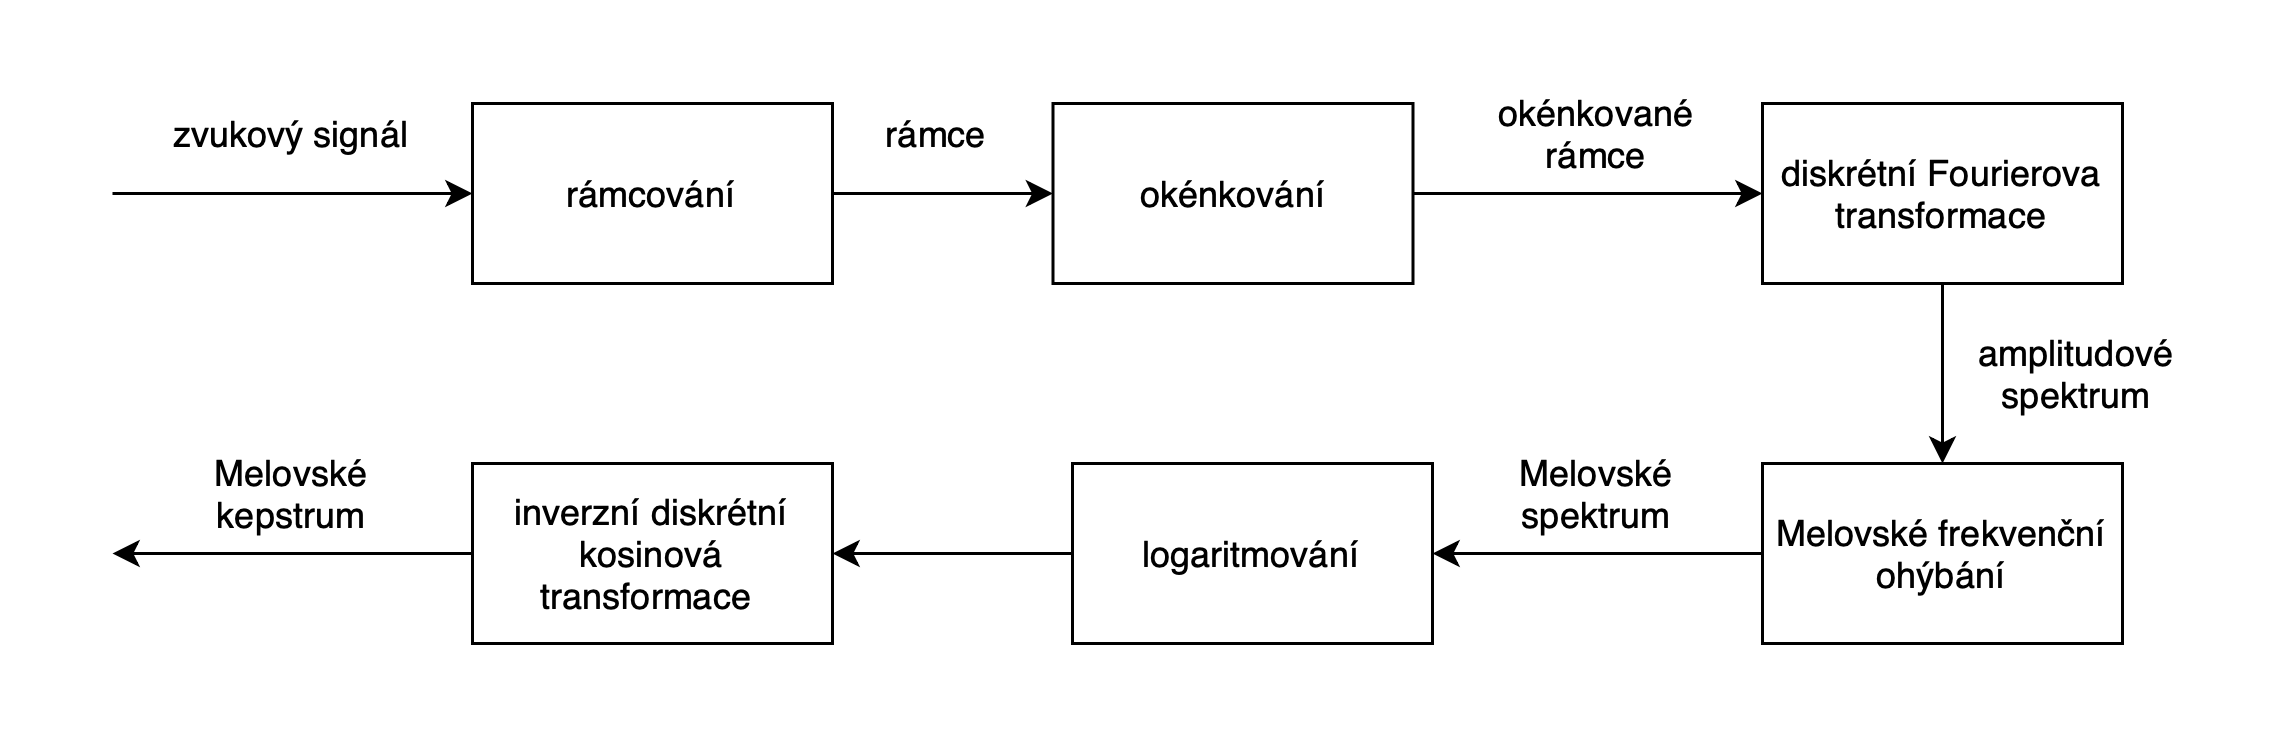
\includegraphics[width=\textwidth,height=\textheight,keepaspectratio]{mfcc_pipeline.png}}
\caption{Postup získání příznaků MFCC}
\label{fig:mfcc_pipeline}
\end{figure}
\FloatBarrier

Při rámcování je zvukový signál je nejprve rozdělen na jednotlivé posuvné rámce. Dále je signál podroben okénkování, kdy je amplituda signálu snížena na konci a na začátku rámce. Může k tomu být použito Hammingovo nebo Hanningovo okénko. Poté je signál převeden pomocí diskrétní Fourierovi transformace (DFT) do frekvenční oblasti. Na výsledné amplitudové spektrum je použito Melovské frekvenční ohýbání. K převodu je použita Melovská banka filtrů složená z trojúhelníkových filtrů s měřítkem v Melovské škále, která zohledňuje vnímaní zvukových frekvencí člověkem. Lidé lépe rozlišují mezi nízkými frekvencemi než mezi vysokými. Dále je signál logaritmován a je provedena inverzní diskrétní kosinová transformace (IDCT). Z koeficientů Melovského kepstra nazývaných také nulté koeficienty lze získat dále koeficienty delta a akcelerační koeficienty (delta delta), které jsou získány použitím první a druhé derivace na nulté koefieficinty \cite{mfcc}.

\section{Způsoby rozpoznávání emocí}
Pro rozpoznávání emocí se používají klasifikátory nebo regresory, které spadají do oblasti strojového učení s učitelem \cite{DBLP:journals/speech/AkcayO20}. Modely strojové učení s učitelem vyžadují označená data. Každý vzorek musí mít přiřazenou anotaci udávající třídu, do které patří. V případě klasifikace jsou to diskrétní štítky, které odpovídají jednotlivým emocím jako jsou na příklad hněv, radost nebo smutek. V případě regrese jsou to desetinné hodnoty, které označují stupeň mocenství, vzrušení nebo dominance většinou v rozsahu od -1 do +1 \cite{konar_chakraborty_2015}.

Často se při klasifikaci ke vzorku přidávají i vzorky z okolí pro zvýšení kontextu, který může zlepšit výsledky rozpoznávaní. Důvodem je, že emoce ovlivňují dlouhodobé charakteristiky řeči. Přesný počet rámců, který by se měl vzít není určen. Na příklad při použít neuronové sítě typu RNN lze pro zachycení kontextu použít kolem maximálně 10 ramců, jinak model začne trpět problémem mizejícího gradientu. Dalším způsobem, jak klasifikovat emoce je podle statických příznaků jako je maximum, minimum nebo časová délka \cite{konar_chakraborty_2015}.

Při trénování se používá často křížová validace, kdy se trénovací a validační sada mění a je vytvořeno několik modelů, kterých výsledky jsou zprůměrovány a je tak dosaženo smysluplnějších výsledkům. U rozpoznávání emocí je používáno především, protože jsou datové sady po většině menšího rozsahu, a tak má rozdělení do jednotlivých sad větší vliv na výsledek. Jako metrika pro ohodnocení modelu se používá přesnost nebo vážená přesnost. Vážená přesnost zohledňuje případný jiný počet vzorků pro každou třídu. Přesnost udává pravděpodobnost, že daný vzorek patří do předpovězené třídy \cite{konar_chakraborty_2015}.

Pro úlohu rozpoznávání emocí v řeči není všeobecně uznaný algoritmus strojového učení, která by se používal. Nicméně nejčastěji používané algoritmy jsou Skryté Markovovy modely (HMM), Gaussian Mixture Model (GMM), Support Vector Machines (SVM), a umělé neuronové sítě (ANN) \cite{DBLP:journals/speech/AkcayO20}.

\chapter{Vybrané základy neuronových sítí}

\section{Vícevrstvý perceptron} % Grammer checked
Vícevrstvý perceptron (MLP) neboli feed-forward neural network je složen z více lineárních vrstev následovaných nelineárními vrstvami. Lineární vrstva se skládá z parametrů vah a biasů a nelineární vrstva je tvořena aktivační funkcí \cite{DBLP:books/lib/Bishop07}.

Aby mohla být neuronová síť označena za hlubokou neuronovou síť, musí mít dvě a více lineárních vrstev. První vrstva modelu se nazývá vstupní vrstvou a poslední vrstvou výstupní. Vrstvy mezi vstupní a výstupní vrstvou jsou označovány jako vrstvy skryté. Každá lineární vrstva má svoji šířku, která určuje počet neuronů ve vrstvě. Při klasifikaci do dvou tříd následuje za výstupní vrstvou funkce sigmoid a při klasifikaci do více tříd je funkce softmax.

\begin{equation}
\label{eqn:sigmoid}
y_j =  \frac{\mathrm{1} }{\mathrm{1} + e^{-x_j} }
\end{equation}

Jako aktivační funkce ve skrytých vrstvách jsou pro MLP používány nejčastěji funkce sigmoid a ReLU. Neuronovou síť typu MLP lze použít také pro regresy, kdy jsou jako aktivační funkce v nelineárních vrstvách umístěny identity \cite{DBLP:books/lib/Bishop07}.

\section{Trénování}
Při trénování neuronové sítě je provedena nejprve dopředná propagace následovaná zpětnou propagací. Po zpětném průchodu sítí jsou parametry sítě upraveny pomocí metody největšího spádu, která minimalizuje ztrátu modelu. Jeden proces učení nazýváme epochou.

Při dopředném průchodu lineární vrstvou jsou vstupní příznaky $ y_i $ přeměněny na výstupní příznaky $ x_j $ pomocí lineární kombinace, kterou lze vyjádřit:

\begin{equation}
\label{eqn:linear_layer}
x_j = b_j + \sum_{i}^{N} y_i w_{ij}
\end{equation}

kde proměnná $ i $ odpovídá indexu příznaku z předchozí vrstvy. $ N $ je celkový počet neuronů předchozí vrstvy. Proměnné $ w_{ij} $ a $ b_j $ reprezentují parametry lineární vrstvy \cite{MATEJU2021327}. Dále jsou příznaky aktivovány nelineární funkcí, kterou lze obecně vyjádřit:

\begin{equation}
\label{eqn:activation}
z_j = h(x_j)
\end{equation}

kde $ x_j $ jsou vstupní příznaky z předchozí vrstvy. Proměnná $ h $ je nelineární, diferencovatelná aktivační funkce a $ z_j $ jsou výstupní příznaky \cite{DBLP:books/lib/Bishop07}.

Proces se opakuje v každé vrstvě sítě. Při dopředném průchodu je nutné si zapamatovat hodnoty vstupních příznaků jednotlivých vrstev sítě, které jsou používány při zpětné propagaci. Výsledkem dopředného průchodu jsou předpovězené hodnoty, z kterých lze pomocí kriteriální funkce získat ztrátu.

Při zpětné propagaci se ztráta modelu propaguje zpět sítí pomocí řetízkového pravidla. Po získání všech gradientů sítě se provede optimalizační algoritmus metody největšího spádu, který aktualizuje parametry sítě. Metodu nejvyššího spádu lze vyjádřit:

\begin{equation}
\label{eqn:gradient_descent}
x_{t+1} = x_t - \alpha \frac{d}{dx}J(x_t)
\end{equation}

kde proměnná $ x_{t+1} $ je hodnota aktualizovaného parametru sítě a $ x_t $ je hodnota původního parametru sítě. Hodnota gradientu pro parametr x je $ \frac{d}{dx} $. Ztráta parametru $ x_t $ je označena $ J $.

\section{Rozdělení na datové sady}
Po získání datové sady je většinou sada rozdělena na tři částí: trénovací, validační a testovací. Trénovací sada je většinou největší a slouží k trénování modelu. Validační a testovací sady jsou menší a slouží k vyhodnocení modelu. Při rozdělování menších datových sad je často použito 70 \% pro trénování, 15 \% pro validaci a 15 \% pro testování. Při rozdělování větších datových sad je možné použít větší část 95 \% pro trénování a zbytek pro validaci a testování. Datová sada je tímto způsobem rozdělena, aby se model naučil dobře zobecňovat. Můžeme to poznat tak, že model dosahuje podobných výsledků na všech datových sadách. Validační datová sada se používá pro zvolení vhodného modelu a příhodných hyperparametrů. Testovací datová sada je použita v posledních částech vývoje modelu, kdy jsou na ní zjištěny konečné výsledky modelu \cite{burkov2019hundred}.

\section{Přeučování a nedoučování}
Při trénování modelu je možné se setkat s nedoučováním a přeučováním. K nedoučování dochází, když model dosahuje nízkých výsledků na trénovací sadě. Nedoučování může být způsobeno na příklad přílišnou jednoduchostí modelu nebo zvolení nevhodných příznaků pro učení. Při přeučování dochází k opačnému jevu, kdy model velice dobře rozpoznává vzorky z trénovací sady, ale velice špatně vzorky ostatní. Mezi hlavní důvody pro vznik přeučování patří přílišná složitost modelu nebo nadměrné množství příznaků ale malou trénovací sadu. Přeučování na datové sadě můžeme poznat na příklad na validanční sadě, kdy ztráta modelu stoupá. Mezi nejčastější techniky používané proti přeučování patří použité jednoduššího modelu, zmenšení počtu vstupních příznaků, přidání trénovacích dat nebo použití regularizace \cite{burkov2019hundred}.

\section{Regularizace}
Regularizace označuje množinu technik, které zabraňují vytvoření příliš složitého modelu. Často jsou používány regularizace typu L1 a L2, které jsou umístěny v algoritmu pro upravovaní parametrů modelu. Je možné použít také techniky, které jsou součástí modelu samotného jako jsou drop out vrstvy nebo vrstvy normalizace dávek \cite{burkov2019hundred}.

\section{Hodnocení výkonu modelu}
Model lze hodnotit podle průběhu ztráty modelu na datových sadách. Pokud ztráta klesá u všech sad, tak je předpoklad, že se model učí správně. Při klasifikace lze použít více metrik a nástrojů pro vyhodnocení modelu. Lze počítat na příklad přesnost, preciznost, úplnost nebo matice záměn.

\subsection{Dropout}
Princip dropout spočívá v náhodném vypínání neuronů ve vrstvě během trénování. Dropout bere jako parametr pravděpodobnost vypnutí jednoho neuronu. Čím vyšší je pravděpodobnost vypnutí, tím je vyšší účinek regularizace \cite{burkov2019hundred}.

\subsection{Normalizace dávky}
Normalizace dávky spočívá v normalizaci výstupu z předešlé vrstvy modelu před vstupem do následující. Použití normalizace může vést k rychlejšímu a stabilnějšímu trénování \cite{burkov2019hundred}. Vztah pro výpočet normalizace dávky lze vyjádřit pomocí následujícího vzorce:

\begin{equation}
\label{eqn:batch_mean}
z_i = \frac{x_i - \mu_b}{\sqrt{\sigma^2_b}}
\end{equation}

kde $ z_i $ je normalizovaný vzorek. Hodnota $ \mu_b $ označuje průměr dávky a $ \sigma^2_b $ znázorňuje rozptyl dávky. Parametr $ x_i $ je jeden vzorek dávky.

\subsection{Matice záměn}
Matice záměn shrnuje výkon modelu. Na jedné z os matice jsou vyobrazeny správné třídy a na druhé jsou třídy předpovězené. Jednotlivé prvky matice záměn udávají počet přiřazených vzorků. Pokud by byly všechny předpovědi správné byly by hodnoty větší než nula na hlavní diagonále matice. Příklad matice záměn pro klasifikaci do dvou tříd je znázorněn na obrázku \ref{fig:conf_matrix-example}.

\begin{figure}[h]
\centerline{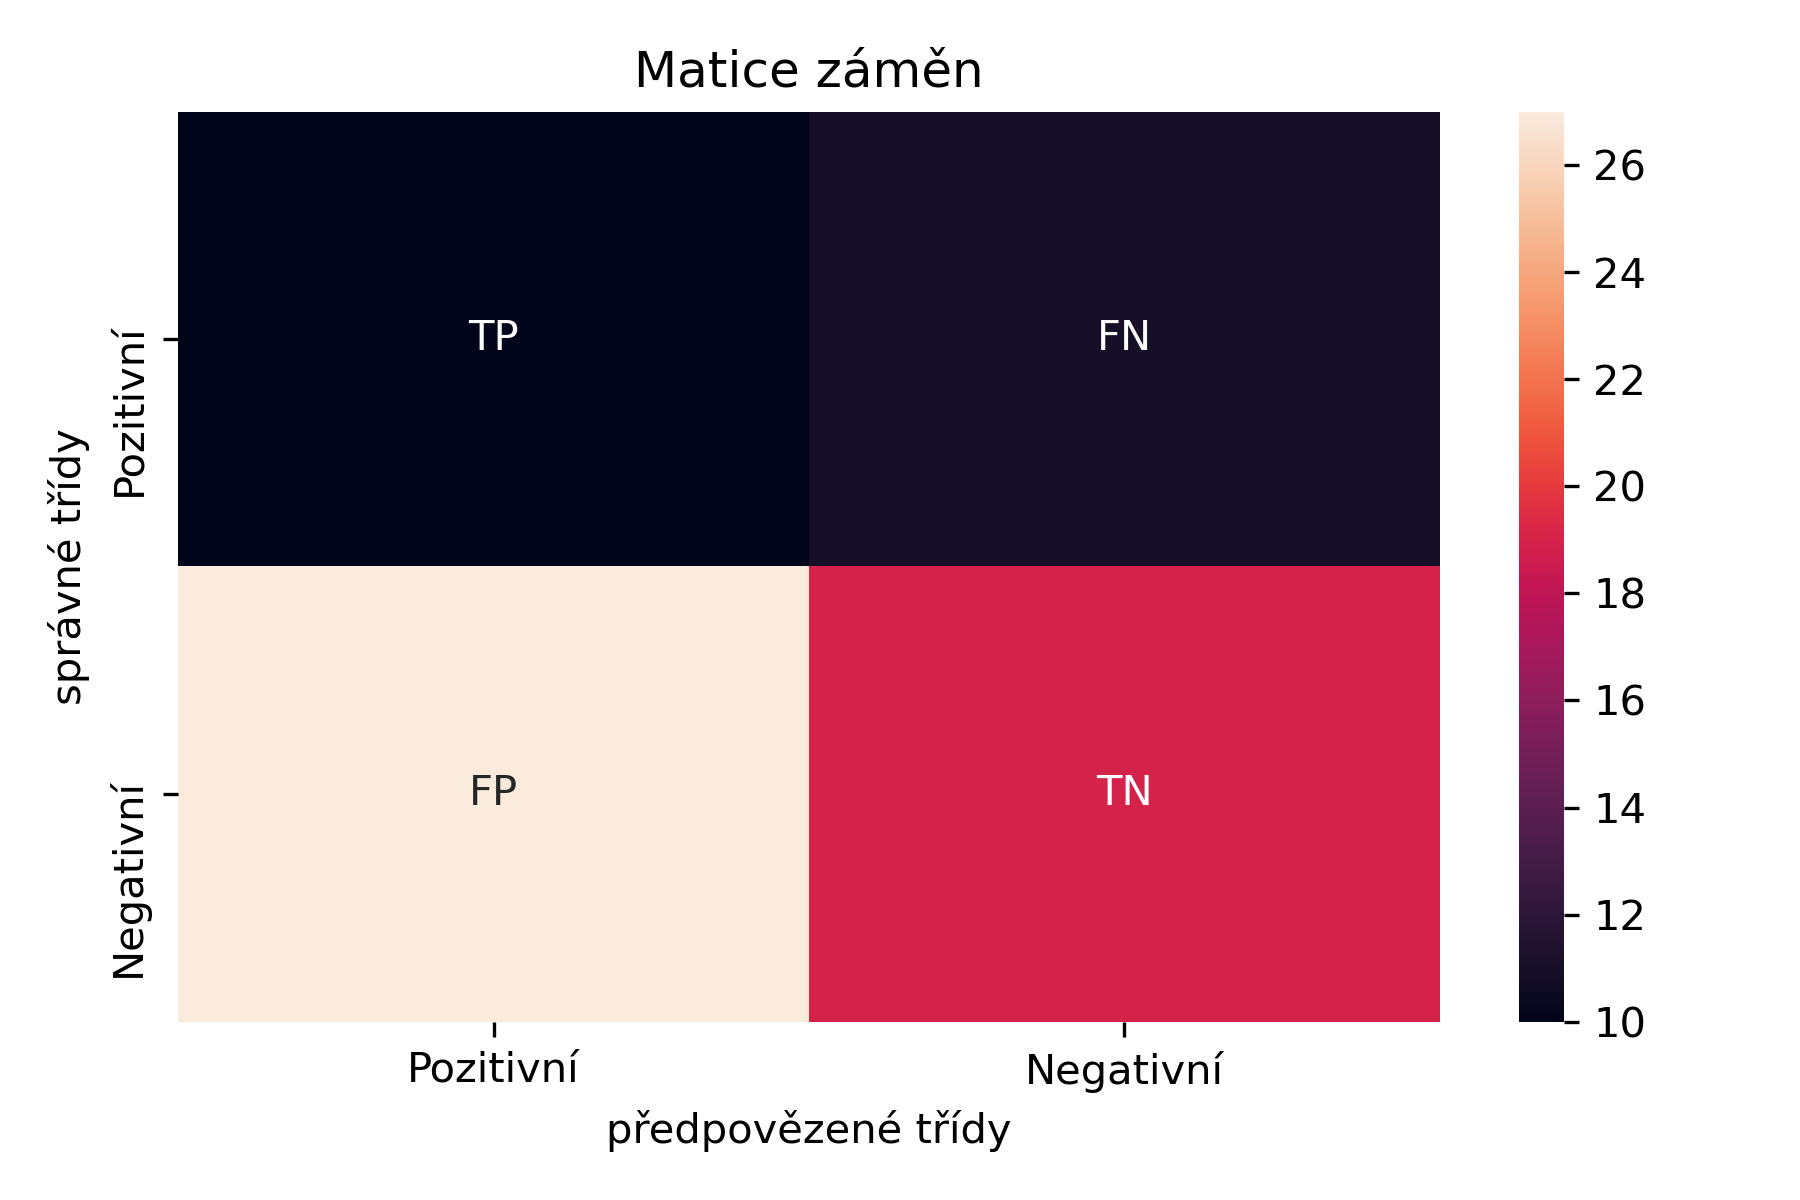
\includegraphics[scale=.7]{conf_matrix-example.png}}
\caption{Matice záměn pro dvě třídy}
\label{fig:conf_matrix-example}
\end{figure}
\FloatBarrier

kde TP a TN jsou počty správně klasifikovaných pozitivních a negativní tříd. FP a FN jsou množství nesprávně přiřazených pozitivních a negativních tříd.

\subsection{Přesnost}
Přesnost udává počet všech správně klasifikovaných vzorků vůči počtu všech vzorků. Často se hodnota násobí sty, aby výsledek vyšel v procentech. Přesnost pro dvě třídy lze znázornit následujícím vzorcem \ref{eqn:accuracy}:

\begin{equation}
\label{eqn:accuracy}
acc = \frac{TP + TN}{TP + TN + FP + FN}
% přesnost = \frac{pravdivé pozitivní + pravdivé negativní}{pravdivé % pozitivní + pravdivé negativní + nepravdivé negativní + pravdivé % negativní}
\end{equation}

kde TP a TN jsou počty správně klasifikovaných pozitivních a negativní tříd. FP a FN jsou množství nesprávně přiřazených pozitivních a negativních tříd. 

\subsection{Hyperparametry}
Hyperparametry jsou parametry ovlivňující učení modelu. Na rozdíl od parametrů modelu se je nelze naučit z trénovacích dat \cite{geron2019hands}. Můžeme je dělit podle toho, jestli jsou používány při návrhu neuronové sítě nebo při samotném trénování. Při návrhu neuronové sítě lze na příklad upravovat počet a šířka skrytých vrstev. Mezi hyperparametry používané při trénování modelu lze zařadit míru učení, počet trénovacích epoch nebo velikost dávky \cite{dagli_2021}.

\section{Vybrané koncepty}

% Vybrané koncepty
\subsection{Křížová entropie} % Grammer checked
Jako kriteriální funkce pro klasifikaci do více tříd lze použít křížovou entropii, která měří rozdíl mezi dvěma rozděleními pravděpodobnosti. Lze ji vyjádřit:

\begin{equation}
\label{eqn:cross_entropy}
l = -{\sum_{c}^{C}t_{c}\log p_{c}}
\end{equation}

kde $ l $ je výsledná ztráta. Index $ c $ odpovídá klasifikovaným třídám a $ C $ je počet tříd. Proměnná $ p $ značí vstupní pravděpodobnosti pro jednotlivé třídy, které dosahují hodnot od nuly do jedné. $ t $ zastupuje skutečné třídy. Nabývá hodnoty jedna pro správnou třídu a hodnoty nula pro nesprávnou třídu. Minimalizací křížové entropie minimalizujeme rozdíl mezi pravděpodobnostním rozdělením trénovacích dat a pravděpodobnostním rozdělením předpovídaných hodnot \cite{brownlee_2020}.

\subsection{ReLU} % Grammer checked
Rectified linear activation function (ReLU) je aktivační funkce, jejíž výstupem je buď nula, pokud je vstup záporný nebo se hodnota vstupu nezmění, pokud je kladný. Lze ji vyjádřit:

\begin{equation}
\label{eqn:relu}
y = max(0, x)
\end{equation}

kde $ y $ jsou výstupní hodnoty. Proměnná $ x $ zastupuje vstupní hodnoty. Neuronové sítě používající tuto funkci se většinou učí snadněji a dosáhnou lepších výsledků. Výhodou této funkce je, že nepodléhá přesycení, kdy jsou velká čísla na příklad u funkce sigmoid změněna na jedna a velmi malá čísla nula. Důsledkem přesycení je, že jsou funkce jako sigmoid nebo tanh velice citlivé na hodnoty okolo jejich středu a méně na odlehlejší hodnoty. Následně se to projeví při trénovaní modelu, kdy může dojít k problému mizejícího gradientu u hlubších neuronových sítí \cite{brownlee_2020_ReLU}.

\subsection{Softmax} % Grammer checked
Softmax je funkce, která přemění vektor čísel na vektor pravděpodobností, kde jsou pravděpodobnosti pro jednotlivé prvky úměrné velikosti všech prvků vektoru. Funkci lze vyjádřit vzorcem:

\begin{equation}
\label{eqn:softmax}
p_i = \frac{e^{s_i}}{\sum_{c}^{C}e^{s_c}}
\end{equation}

kde $ p_i $ je hodnota výstupní pravděpodobnosti. Proměnná $ s $ odpovídá skóre výstupní vrstvy neuronové sítě. Hodnoty $ i $ a $ c $ odpovídají indexu příchozího skóre a $ C $ počtu klasifikovaných tříd. Součet všech výsledných pravděpodobností je roven jedné. Funkce se používá při klasifikaci do více tříd a stojí na konci klasifikátoru. Každá výstupní pravděpodobnost odpovídá jednotlivé třídě datové sady \cite{brownlee_2020_Softmax}.

\chapter{Vývoj balíčku pro rozpoznávání emocí} % Grammer checked
Byl vytvořen balíček s moduly pro rozpoznávání emocí. Balíček je napsán v jazyku Python verze 3. Mezi vytvořené moduly patří: convertors pro převod dat, data pro práci s daty, classifiers na tvorbu klasifikátoru, files na práci se soubory, datasets k tvorbě datových sad, prepare pro přípravu datových sad a train sloužící k trénování modelu. Modely jsou psány objektově. Byly použity knihovny a frameworky: PyTorch 1.6 pro tvorbu a trénování modelu, seaborn 0.11 a matplotlib 3.3 pro vytvoření grafů, logging 0.4 pro logování při trénování modelu, scikit-learn 0.23 pro rozdělení dat na sety, pandas 1.1 numpy 1.18 pro ukládání a práci s daty, os a sys pro práci s operačním systémem, re pro parsování anotací, subprocess pro spouštění příkazů z příkazové řádky, PyHTK pro načítání souborů vytvořené pomocí sady nástrojů HTK.

\section{Výběr datových sad} % Grammer checked
Hlavním kritériem při výběru byla dostupnost datové sady, proto byly vybrány sady bezplatné a dostupné pro vědecké účely. Byly vybrány datové sady především anglické: RAVDESS, TESS a SAVEE a jedna italská: EMOVO. Datové sady mají společných sedm emocí, mezi které patří emoce: neutrální, hněv, strach, smutek, spokojenost, odpor a překvapení. Současně mají společně zastoupeny obě pohlaví. Informace o datových sadách byly shrnuty v tabulce \ref{tab:overview}).

\begin{table}[ht]
\centering
\resizebox{\textwidth}{!}{\begin{tabular}{ccccccc}
  \hline
 název & jazyk & počet tříd & počet mluvčích & pohlaví mluvčích & počet promluv & celková délka (hodiny) \\
  \hline
    RAVDESS & angličtina & 8 & 24 & obě & 1440 & 1.5 \\
    SAVEE   & angličtina & 7 & 4  & muži  & 480  & 0.5 \\
    TESS    & angličtina & 7 & 2  & ženy  & 2800 & 1.6 \\
    EMOVO   & italština  & 7 & 6  & obě & 588  & 0.5 \\
   \hline
\end{tabular}}
\caption{Přehled vybraných datových sad}
\label{tab:overview}
\end{table}
\FloatBarrier

Celkem tedy byly získány čtyři datové sady o dvou jazycích se zastoupením sedmi emocemi. Dohromady vzniklá datová sada má celkem přibližně dobu trvání čtyř hodin.

\section{Předpříprava dat} % Grammer checked
Data byla nejdříve předzpracována. Byl sjednocen jejich formát a data převedena na příznaky MFCC. Formát byl sjednocen pomocí nástroje Fast Forward MPEG (FFmpeg) přístupného z příkazové řádky. Nahrávky byly převedeny na vzorkovací frekvenci 16 kHz a byl zachován jeden zvukový kanál. Zvukové nahrávky byly převedeny pomocí příkazu na obrázku \ref{fig:ffmpeg}.

\begin{figure}[htbp]
\centerline{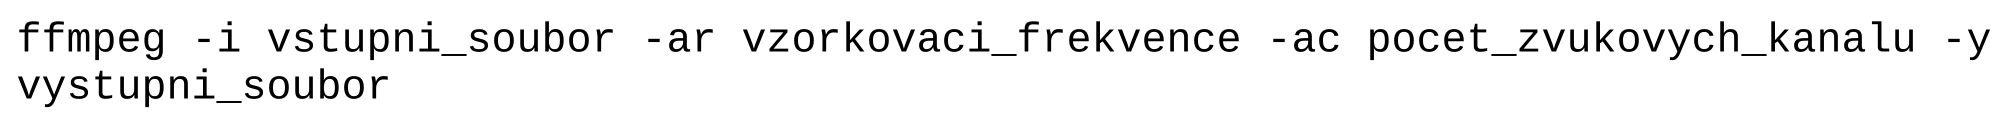
\includegraphics[width=\textwidth,height=\textheight,keepaspectratio]{ffmpeg_command.png}}
\caption{Příkaz FFmpeg}
\label{fig:ffmpeg}
\end{figure}
\FloatBarrier

Dále byly nahrávky převedeny na MFCC příznaky. K převodu byla použita sada nástrojů Hidden Markov Model Toolkit (HTK). Pro převod byl použit konfigurační soubor (viz Obr. \ref{fig:htk_config}).

\begin{figure}[htbp]
\centerline{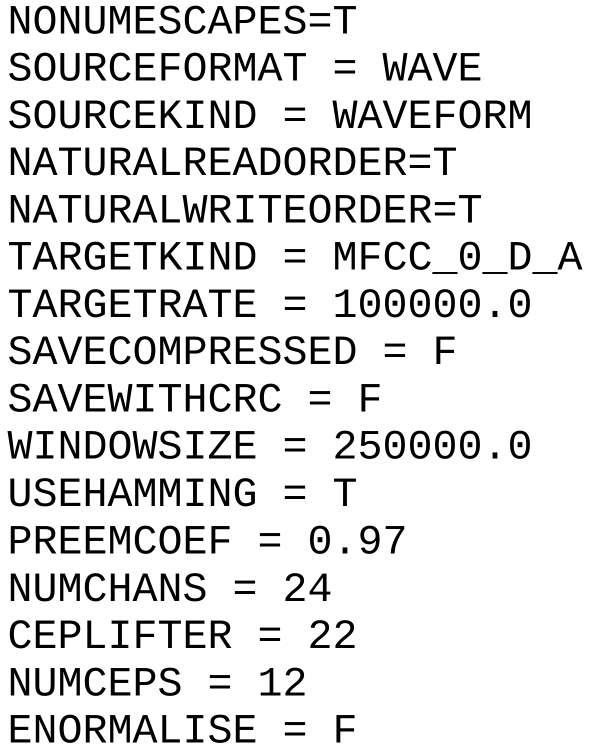
\includegraphics[scale=.2,keepaspectratio]{htk_config.png}}
\caption{Konfigurační soubor}
\label{fig:htk_config}
\end{figure}
\FloatBarrier

MFCC formát byl zvolen jako MFCC\_0\_D\_A, kde chceme získat nulté, delta a akcelerační koeficienty. Dále lze vyčíst, že pro okénkování byla použita Hammingova okénkovací funkce a velikost okénka byla nastavena na 25 ms. Převod byl uskutečněn pomocí příkazu HCOPY na obrázku \ref{fig:htk}.

\begin{figure}[htbp]
\centerline{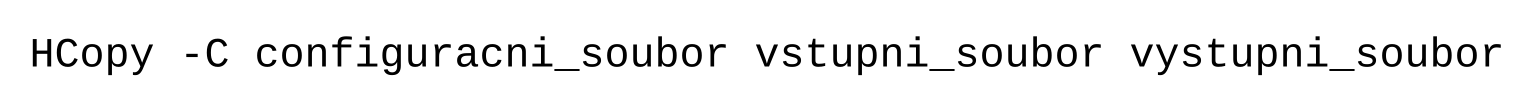
\includegraphics[width=\textwidth,height=\textheight,keepaspectratio]{htk_command.png}}
\caption{Příkaz HTK}
\label{fig:htk}
\end{figure}
\FloatBarrier

Třídy pro převod byly implementovány v modulu conversors. Byla vytvořena základní třída Convertor, z které konkrétní převaděče dědí. Pro sjednocení formátu byla vytvořena třída AudioFormatConverter a třída MFCCConverter pro převod na příznaky MFCC. Vztahy mezi převaděči jsou znázorněny na UML diagramu \ref{fig:convertor}.

\begin{figure}[ht]
\centerline{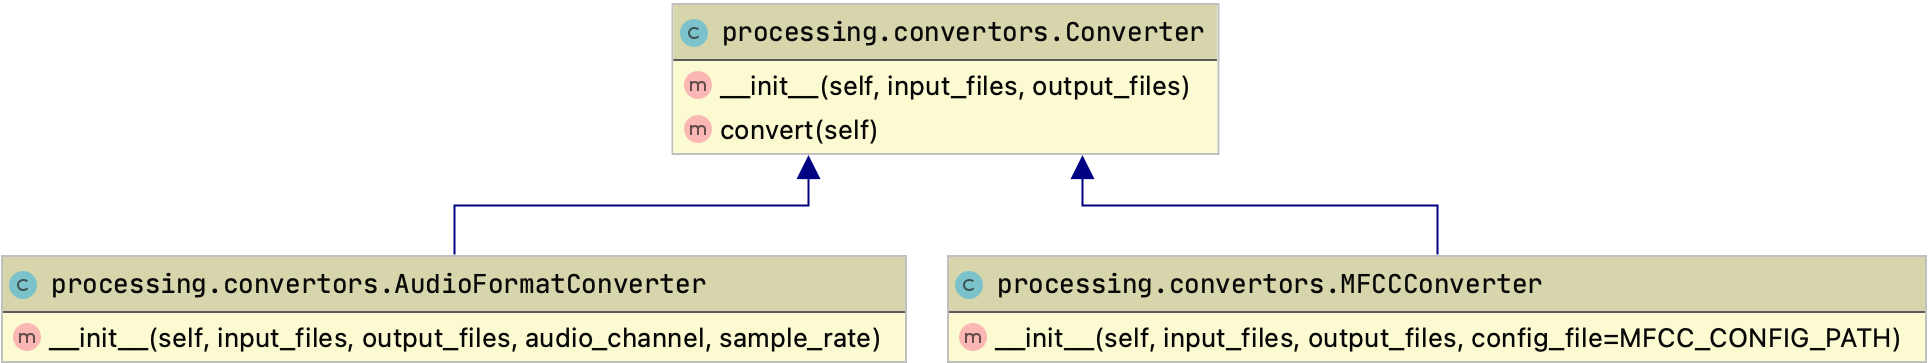
\includegraphics[width=\textwidth,height=\textheight,keepaspectratio]{convertors.png}}
\caption{Třídy Converter}
\label{fig:convertor}
\end{figure}
\FloatBarrier

\section{Příprava datových sad pro trénování} % Grammer checked
Pro načítání dat byla vytvořena třída Dataset v modulu data. Hlavními úkoly této třídy bylo načíst data a z anotací získat třídy emocí. Třída Dataset dědí od třídy Directory z modulu files, která umožňuje získat cesty k souborům ve složce. Vztah mezi třídami je znázorněn na diagramu \ref{fig:datasets}.

\begin{figure}[h!]
\centerline{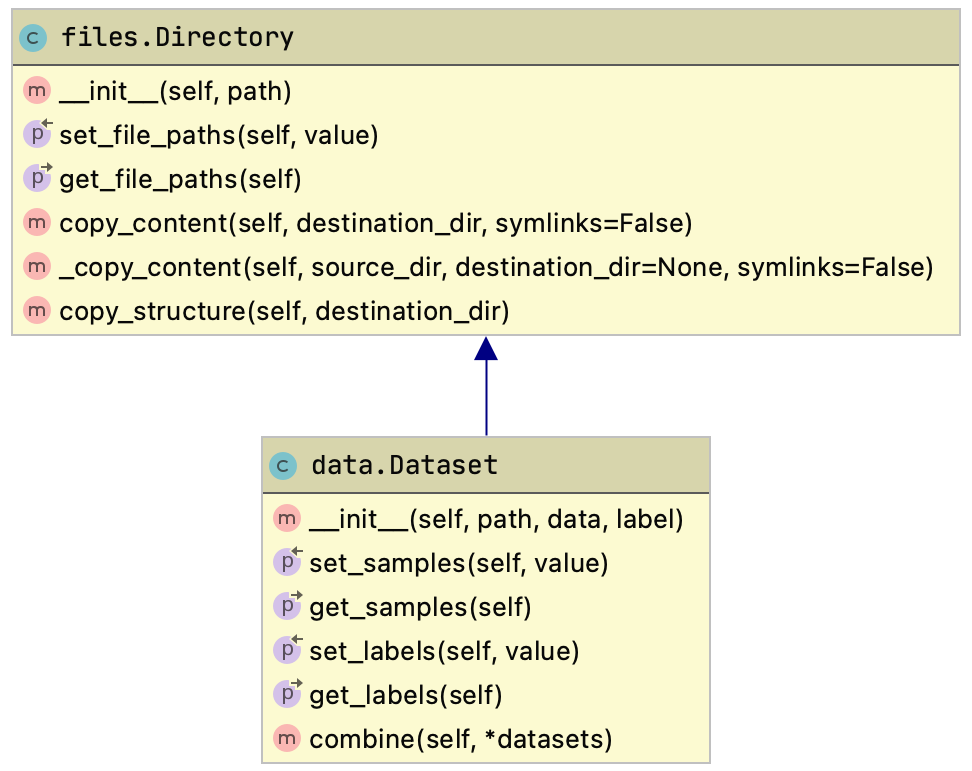
\includegraphics[scale=.25,keepaspectratio]{data-dataset.png}}
\caption{Třída Dataset}
\label{fig:datasets}
\end{figure}
\FloatBarrier

Třída Dataset má navíc atributy samples pro uložení načtených vzorků a labels pro uložení anotací pro vzorky. Při vytváření objektu třídy Dataset jsou předávány objekty třídy Data a Label. Objekt třídy Data načte na základě cesty k souboru vzorek a Label z anotace získá informace potřebné k vytvoření anotace pro vzorek. Jelikož jsou datové sady odlišně značeny, byly vytvořeny třídy dědící od třídy UnifiedLabel (viz Obr. \ref{fig:label}), které navíc anotace pro vzorek převedly na stejné značení.

\begin{figure}[h]
\centerline{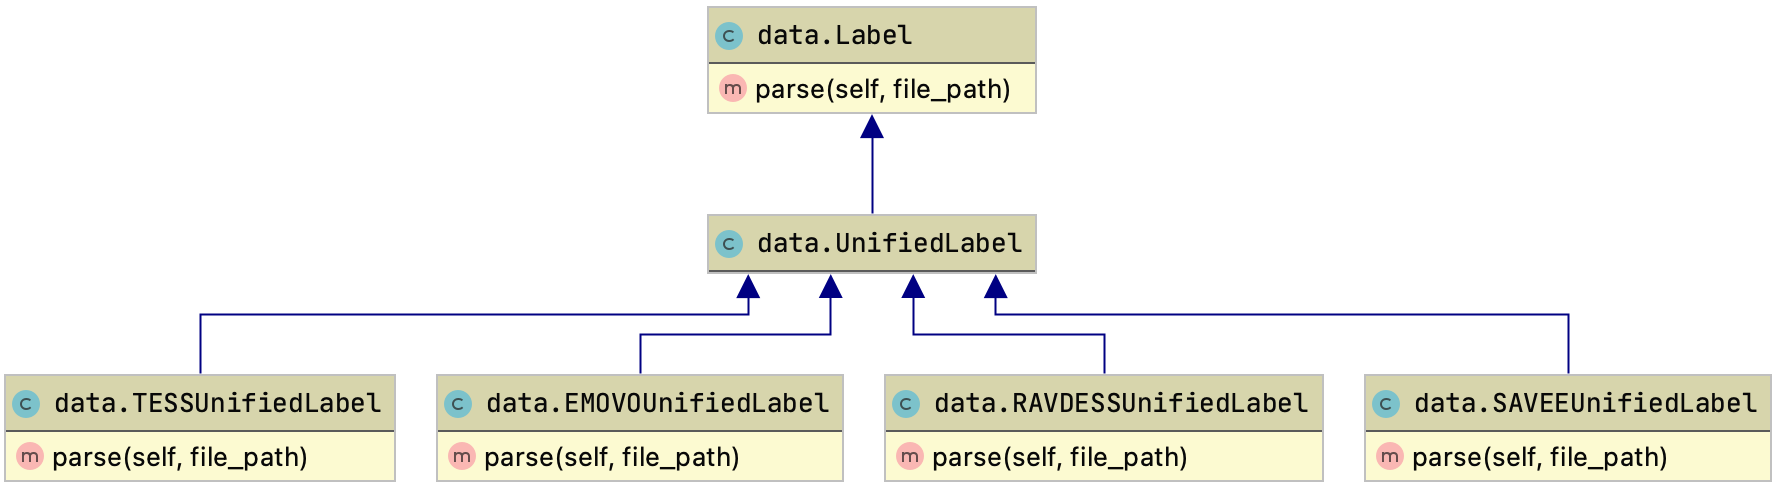
\includegraphics[scale=.25,keepaspectratio]{data-label.png}}
\caption{Třídy Label}
\label{fig:label}
\end{figure}
\FloatBarrier

Z třídy Data (viz Obr. \ref{fig:data}) dědí třída MFCCData umožňující načtení příznaků MFCC a WAVData zprostředkovávající načtení nahrávek ze souboru typu WAV. MFCCData používá třídu HTKFile z balíčku PyHTK pro načtení příznaků.

\begin{figure}[h]
\centerline{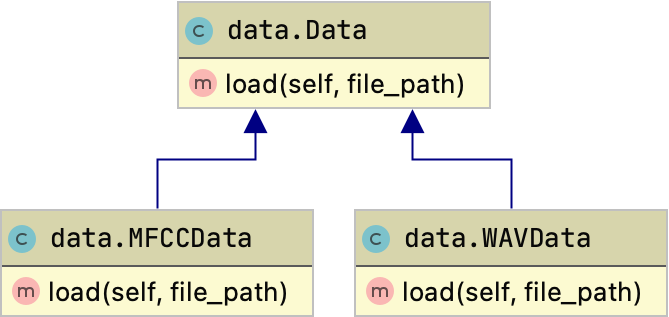
\includegraphics[scale=.25,keepaspectratio]{data-data.png}}
\caption{Třídy Data}
\label{fig:data}
\end{figure}
\FloatBarrier

Dále byla data rozdělena do trénovacích, validačních a testovacích setů. Pro rozdělení byla použita třída Preparer (viz Obr. \ref{fig:preparer}) z modulu prepare. Data byla nejdříve načtena pomocí objektů třídy Dataset. Mohla být sloučena dohromady. Na příklad mohla být vytvořena datová sada ze všech anglických datových sad. Data získaná z objektu Dataset mohla být rozdělena do trénovacího, testovacího a validačního setu. Rozdělení probíhalo rovnoměrně pomocí funkce train\_test\_split z modulu sklearn.model\_selection a vzorky byly rozděleny po celých nahrávkách. Při rozdělování na sety byla zvolena možnost stratify, která rozdělila vzorky rovnoměrně do vzniklých setů podle anotací.

\begin{figure}[h]
\centerline{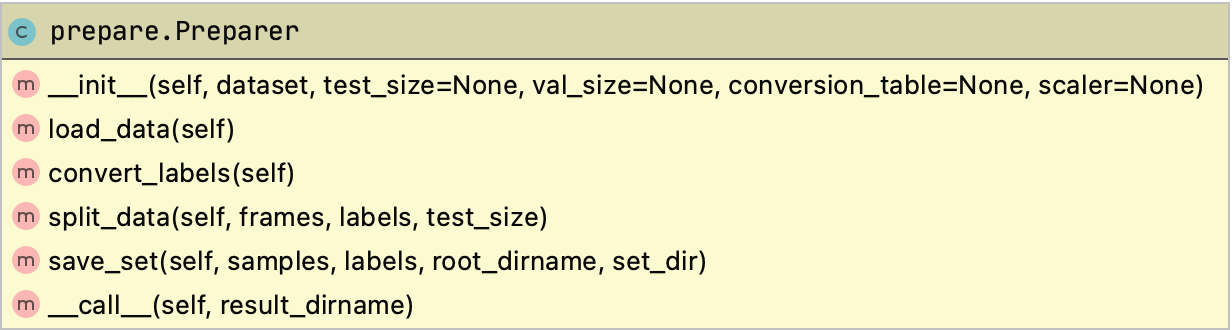
\includegraphics[scale=.25,keepaspectratio]{prepare.png}}
\caption{Třída Preparer}
\label{fig:preparer}
\end{figure}
\FloatBarrier

Jako poslední byly sety uloženy do složky. Každému setu byla přiřazena vlastní složka, která obsahovala soubory labels.npy, samples.py a info.txt. V souboru info.txt byly uloženy informace pro načítání datového setu. Struktura složky je znázorněna na obrázku \ref{fig:file_structure}. Pro ukládání a načítání informací ze souborů info.txt byly vytvořeny třídy DatasetInfoFile (viz Obr. \ref{fig:info_files}) a SetInfoFile. V souboru třídy DatasetInfoFile byly uloženy údaje o počtu příznaků, počtu tříd a počtu vzorků datové sady. Do SetInfoFile byly ukládány počty vzorků, délky vzorků a názvy souborů se vzorky a anotacemi. Data pro rozpoznávání byla uložena ve dvourozměrném poli z balíčku numpy.

\begin{figure}[h]
\centerline{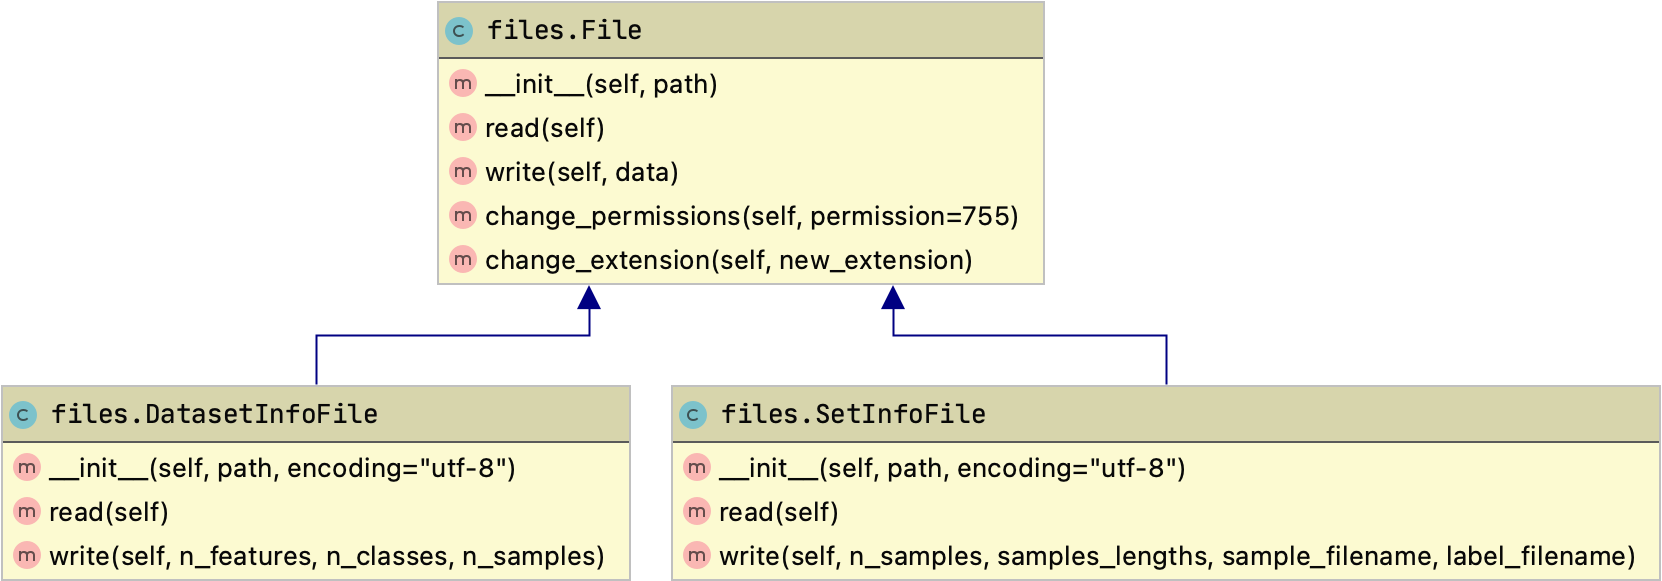
\includegraphics[scale=.25]{files-info.png}}
\caption{Třídy InfoFile}
\label{fig:info_files}
\end{figure}
\FloatBarrier

\begin{figure}[h]
\centerline{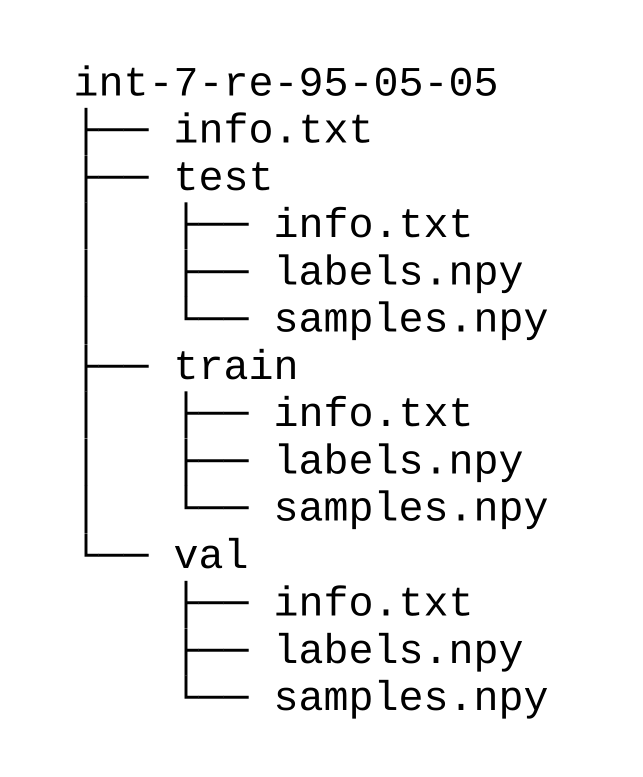
\includegraphics[scale=.22]{dataset_file_structure.png}}
\caption{Souborová struktura uložené datové sady}
\label{fig:file_structure}
\end{figure}
\FloatBarrier

\section{Načítání dat} % Grammer checked
Pro načítání uložených datových sad byl vytvořen objekt NumpyDataset, který dědí od objektu Dataset z balíčku torch.utils.data. Objektu je přidělena cesta k datové sadě. Z textového souboru info.txt si přečte informace potřebné k načtení dat. Mezi důležité parametry, které objekt NumpyDataset při svém vytvoření přebírá, patří velikosti pravého a levého okolí vzorku. Při načtení vzorků ze souboru samples.py jsou ke vzorkům na začátku a na konci přiřazeny okraje, které mají velikosti pravého a levého okolí. Okraje jsou vytvořeny z kopií krajních vzorků a slouží pro zjednodušení výběrů vzorků. Vzorky jsou uloženy popořadě po jednotlivých nahrávkách. Objekt si ukládá indexy začátku a konce nahrávek. Načtené anotace z připravené datové sady odpovídají jednotlivým nahrávkám, proto jsou anotace roztaženy tak, aby odpovídaly délce vzorků nahrávky. Uložení vzorků v objektu NumpyDataset je znázorněno na diagramu \ref{fig:data_arrangement}.

\begin{figure}[htbp]
\centerline{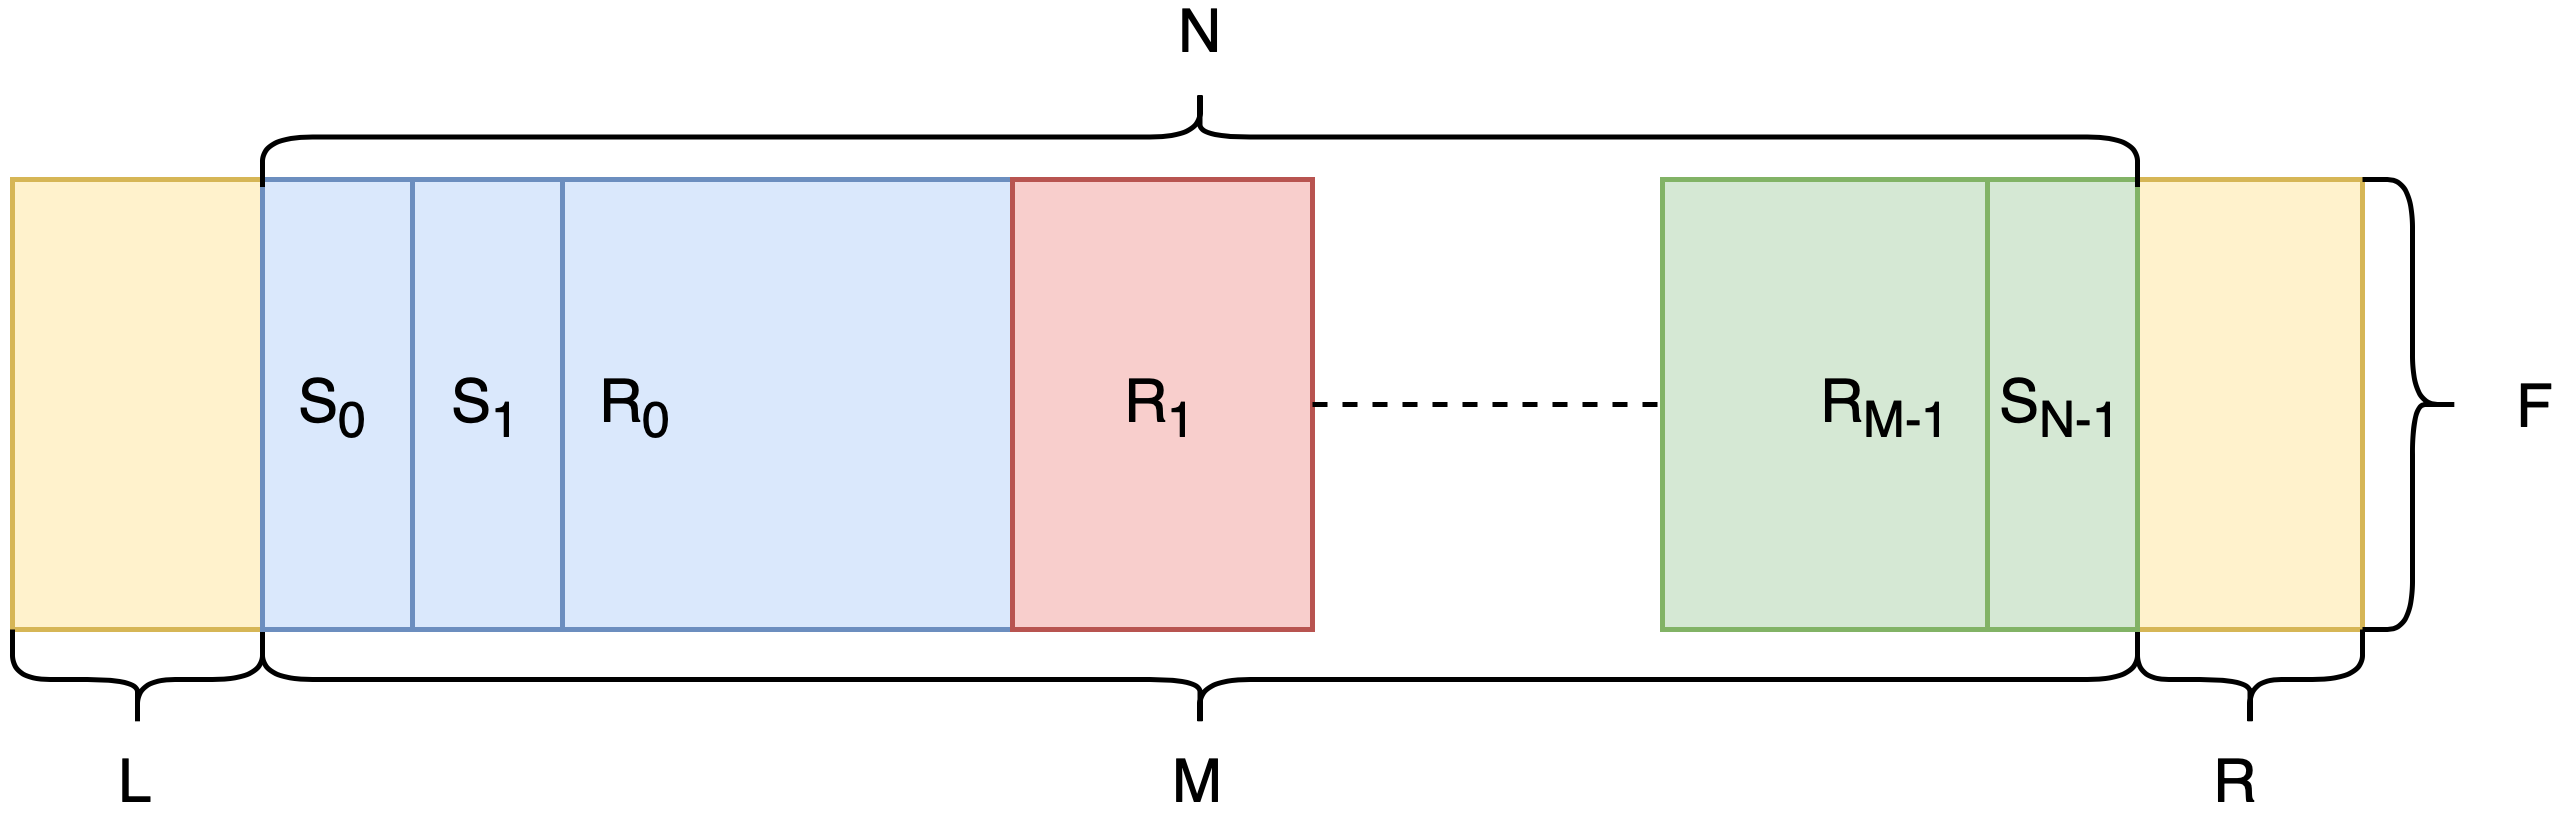
\includegraphics[scale=.125]{dataset_arrangement.png}}
\caption{Uspořádání dat v NumpyDatasetu}
\label{fig:data_arrangement}
\end{figure}
\FloatBarrier

kde písmenem $ S $ jsou označeny jednotlivé vzorky. $ R $ označuje jednotlivé nahrávky, které mohou mít různou délku. Písmeno $ N $ udává počet vzorků a $ M $ počet uložených nahrávek. $ L $ a $ R $ značí velikost pravého a levého okraje. Písmeno $ F $ odpovídá počtu příznaků pro jeden vzorek.

Z třídy NumpyDataset dědí třídy NumpyFrameDataset a NumpySampleDataset (viz Obr. \ref{fig:numpy_dataset}), které se liší v implementaci metod \_\_len\_\_ a \_\_getitem\_\_. Metoda \_\_len\_\_ při zavolání vrací délku datové sady, která u třídy NumpyFrameDataset odpovídá počtu vzorků a u třídy NumpySampleDataset odpovídá počtu nahrávek. Metoda \_\_getitem\_\_ vrací jeden vzorek z Datasetu, u třídy NumpyFrameDataset vrací metoda jeden vzorek a třídy NumpySampleDataset vrací jednu nahrávku. Třída NumpyDataset je tímto způsobem rozdělena. Důvodem pro rozdělení je, že při načítání dat pro validaci můžeme pomocí třídy NumpySampleDataset spočítat přesnost na celou nahrávku. Naopak při trénování je potřeba načítat vzorky po dávkách, které mají fixní délku na rozdíl od nahrávek, u kterých se délka mění. Vzorky se při trénování často míchají, a to je také důvod, proč je lepší mít třídu rozdělenou.

\begin{figure}[h]
\centerline{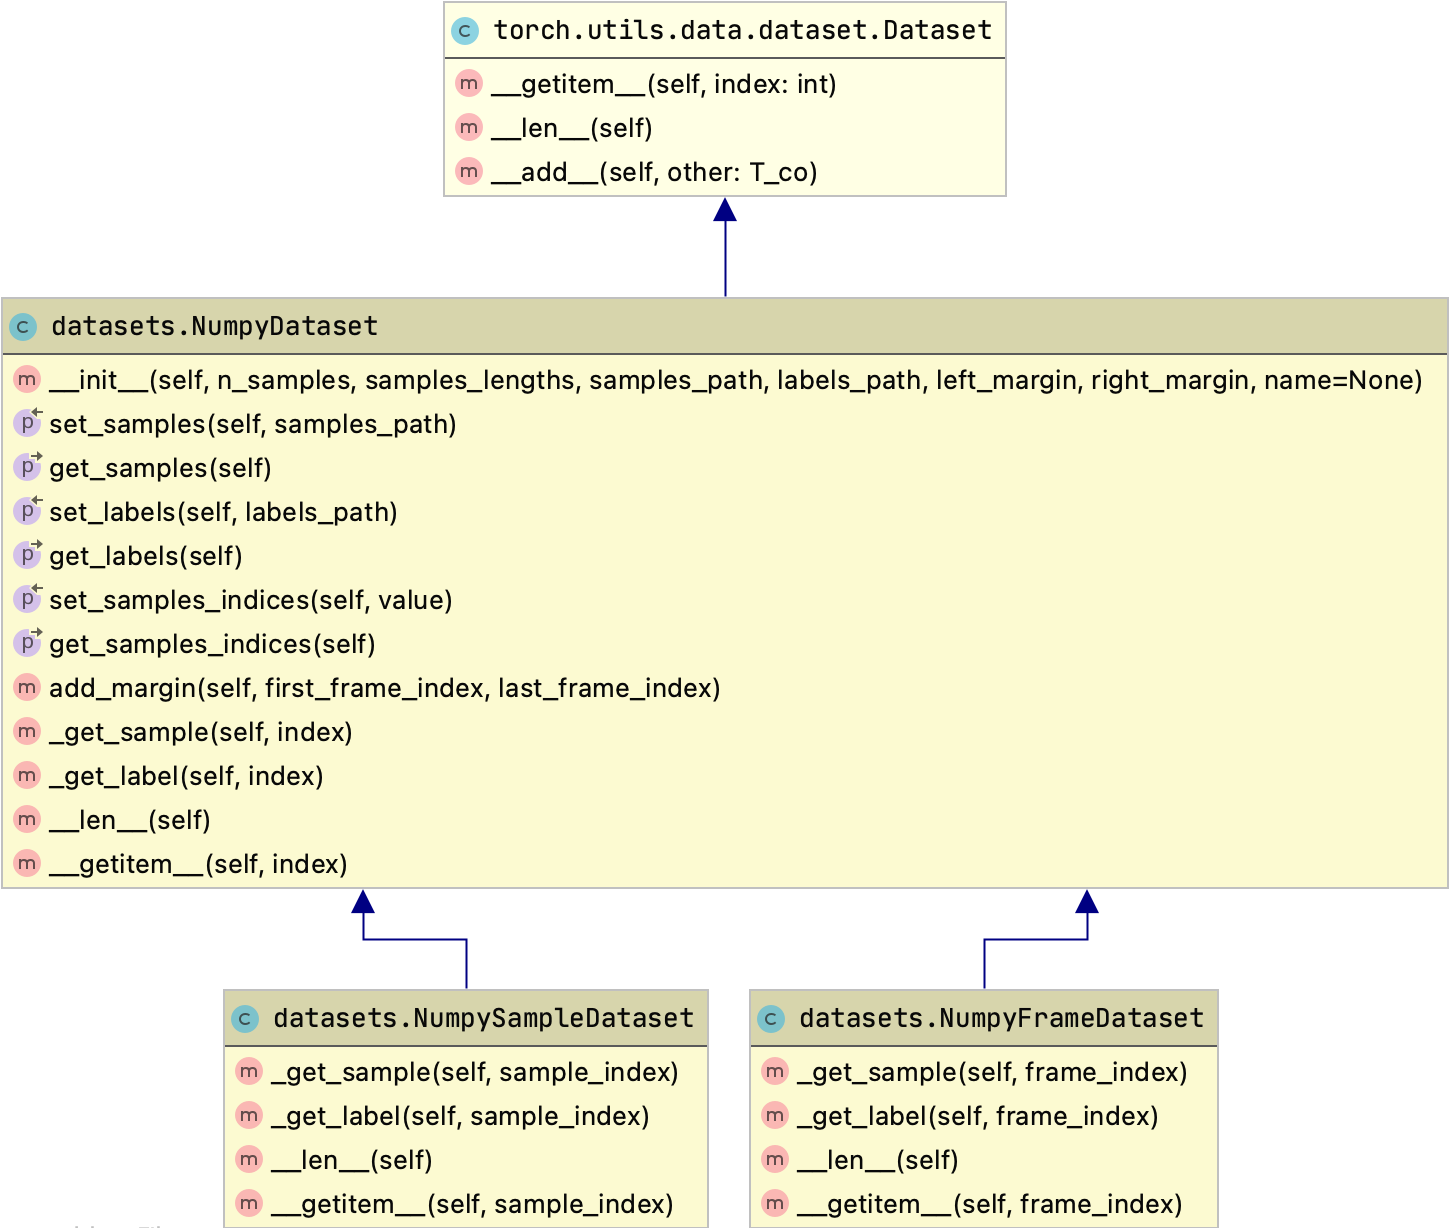
\includegraphics[scale=.185]{datasets.png}}
\caption{Třídy NumpyDataset}
\label{fig:numpy_dataset}
\end{figure}
\FloatBarrier

Ke vzorkům jsou při výběru přidávány vzorky z okolí pro větší zachycení kontextu nahrávky. Počet vzorků z okolí je načítán na základě velikosti pravého a levého okraje. Vybrané vzorky jsou před vrácením zploštěny. Proces výběru vzorku je znázorněn na obrázku \ref{fig:sample_selection}.

\begin{figure}[h]
\centerline{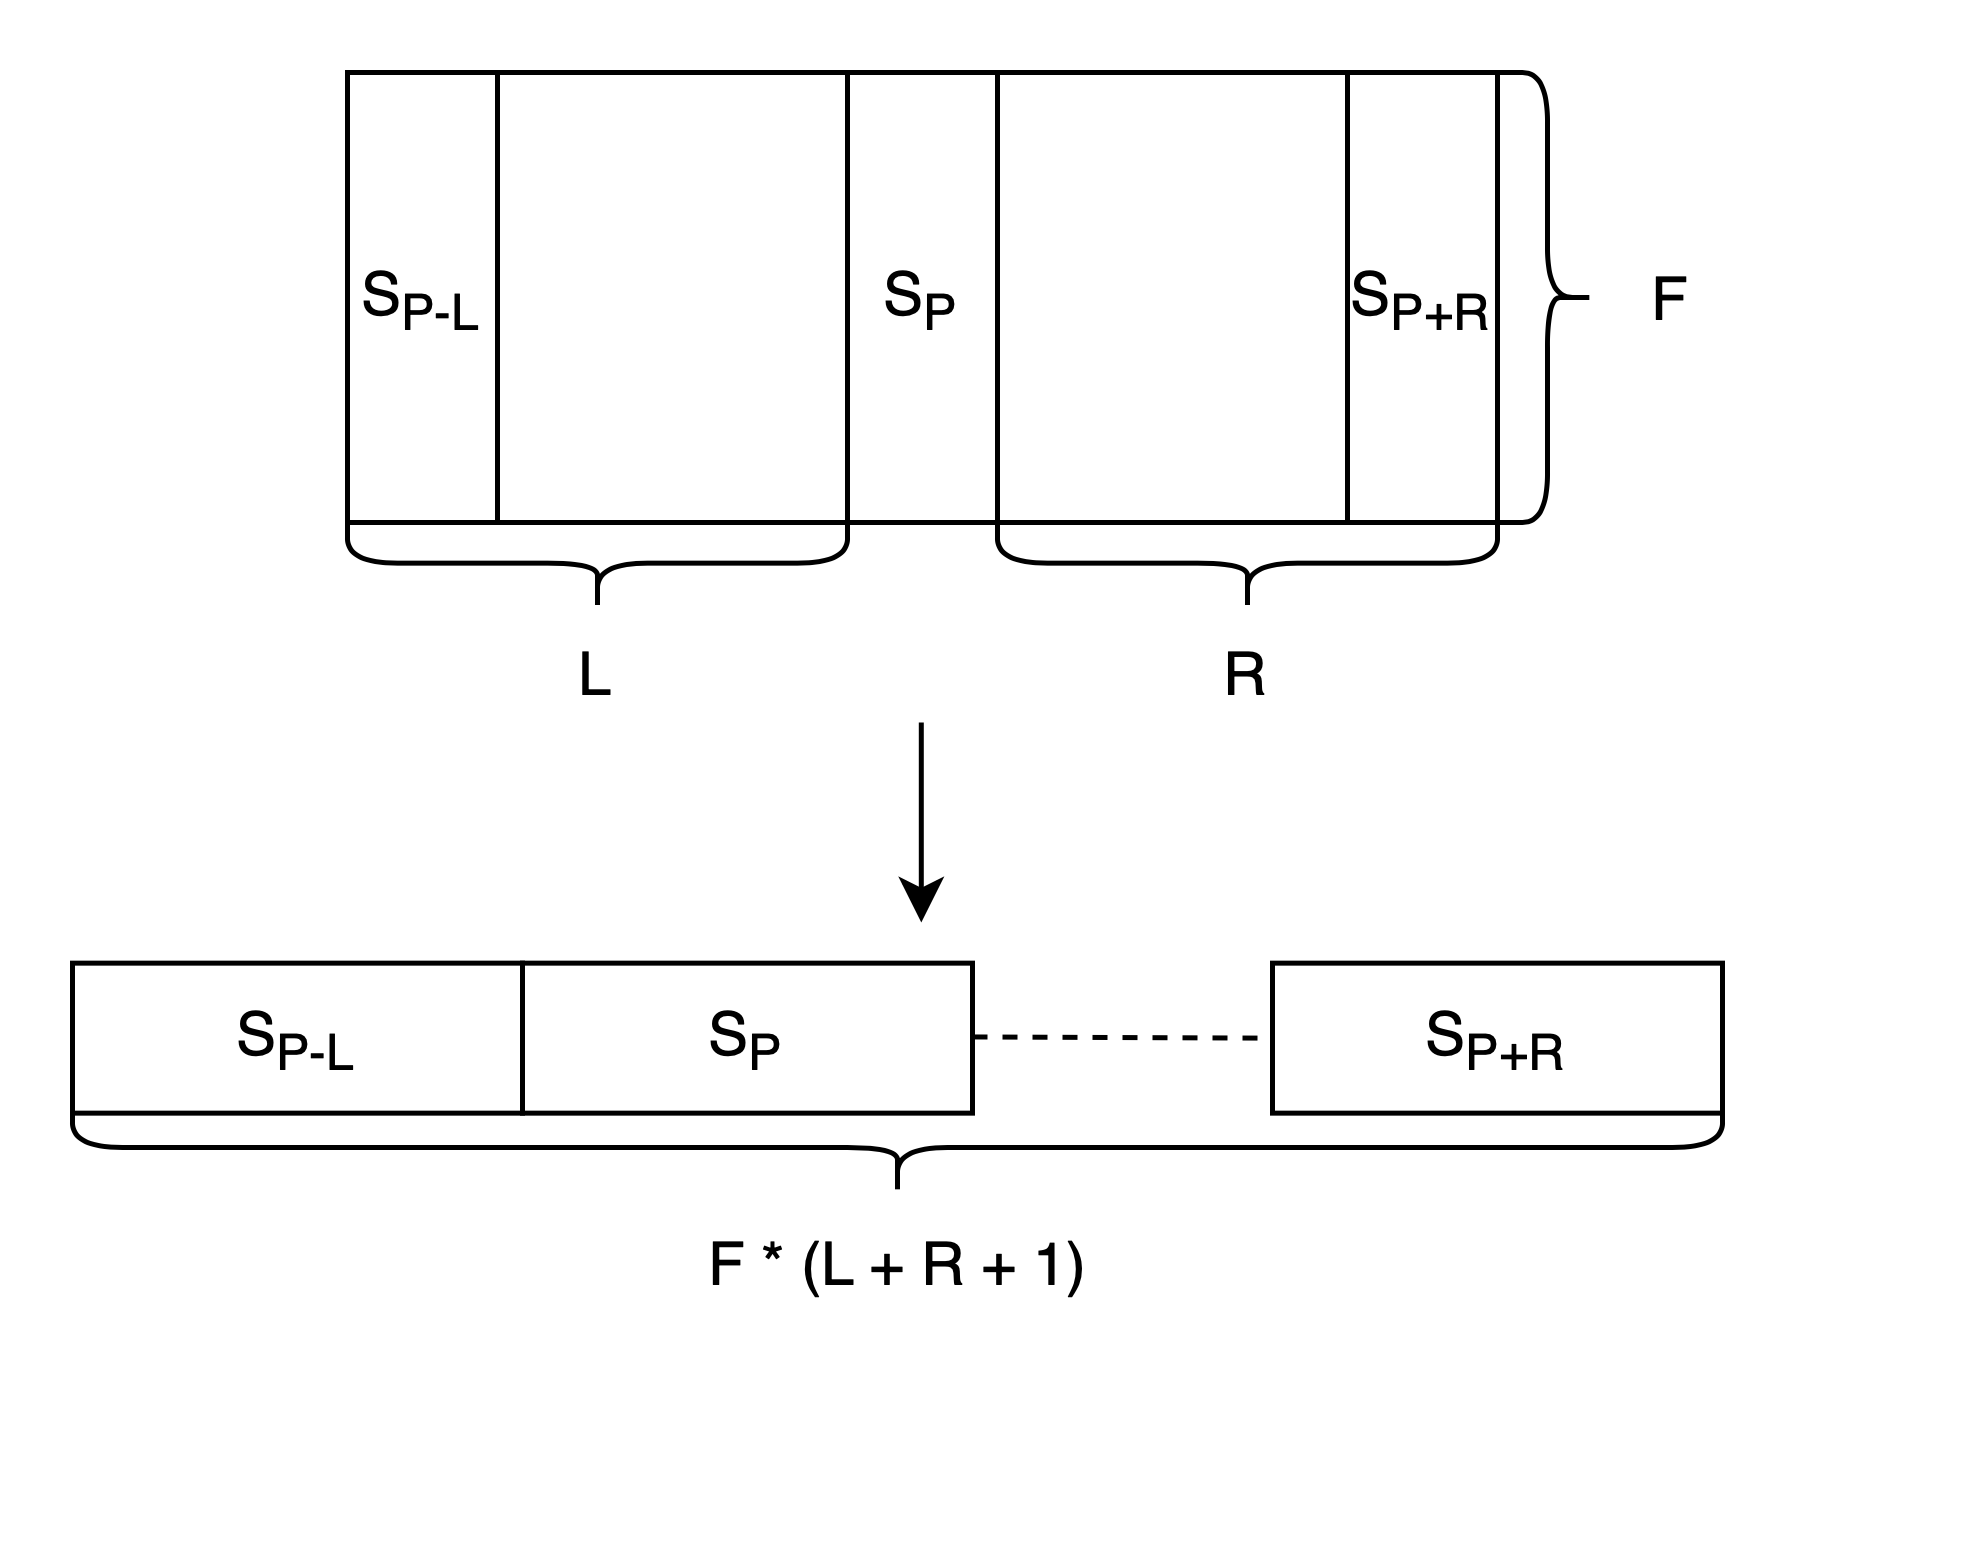
\includegraphics[scale=.125]{sample_selection.png}}
\caption{Výběr vzorku}
\label{fig:sample_selection}
\end{figure}
\FloatBarrier

kde vybraný vzorek má označení $ S $ a krajní vzorky mají označení $ S_{P-L} $ a $ S_{P+R} $. Písmeno $ F $ označuje počet příznaků pro jeden vzorek. Značky $ L $ a $ P $ odpovídají délkám levého a pravého okraje. Výsledný zploštělí obrázek má délku odpovídající $ F * (L + R + 1) $.

\section{Tvorba neuronové sítě}
Byl vytvořen model FeedForwardNet pomocí dědění z třídy Module z modulu torch.nn. V konstruktoru třídy FeedForwardNet byly vytvořeny jednotlivé vrsty neuronové sítě a byly uloženy do objektu ModuleList z modulu torch.nn. Dále byl pomocí metody forward implementován dopředný průchod.

\subsection{Trénování}
V modulu train byla vytvořena třída Trainer (viz Obr. \ref{fig:trainer}), jejíž úkolem je trénování modelu. Hlavní parametr předaný při vytváření instance třídy je model. Dále jsou předány trénovací, testovací a validační sady. Pro trénování modelu jsou důležité parametry optimizer k úpravě parametrů a kritérium pro získání ztráty. Parametr device umožňuje zvolit zařízení, na kterém bude trénování probíhat. Jako poslední je předán objekt typu Stats (viz Obr. \ref{fig:stats}), do kterého se ukládají statistiky získané při trénování modelu. 

\begin{figure}[ht]
\centerline{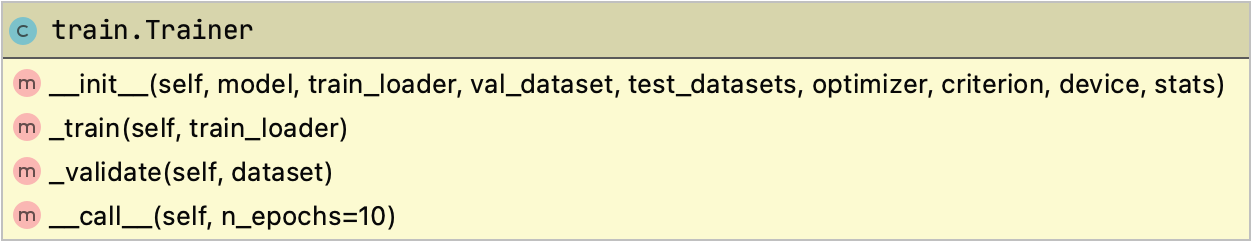
\includegraphics[scale=.3]{train-trainer.png}}
\caption{Třída Trainer}
\label{fig:trainer}
\end{figure}
\FloatBarrier

\begin{figure}[ht]
\centerline{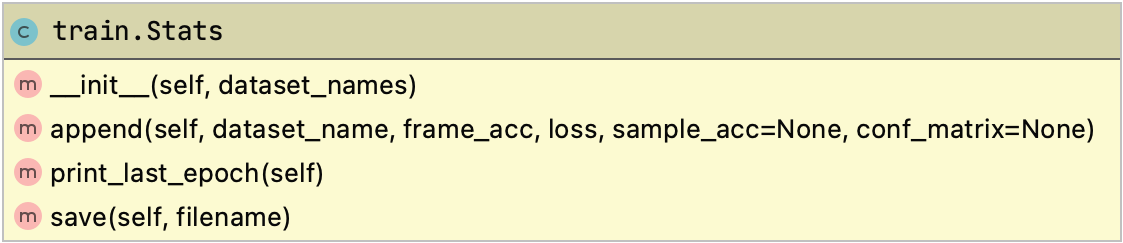
\includegraphics[scale=.33]{train-stats.png}}
\caption{Třída Stats}
\label{fig:stats}
\end{figure}
\FloatBarrier

Trénování je zahájeno zavoláním objektu třídy Trainer, kdy je předán počet trénovacích epoch. Každou epochu jsou do objektu třídy Stats ukládány statistiky trénování, mezi které patří přesnost na jeden vzorek, přesnost na jednu nahrávku, ztráta modelu a matice záměn. Řádky matice záměn odpovídají správným třídám a sloupce odpovídají předpovězeným třídám. Jednotlivé prvky matice odpovídají počtu přiřazených vzorků ke třídě. Pokud by byly všechny vzorky přiřazeny správně, tak by byla všechna čísla větší než nula na hlavní diagonále matice. Zároveň jsou vybrané statistiky vypisovány v přehledném výpisu (viz Obr. \ref{fig:print}) do konzole, k výpisu je používán objekt třídy StatsPrinter (viz Obr. \ref{fig:printer}).

\begin{figure}[ht]
\centerline{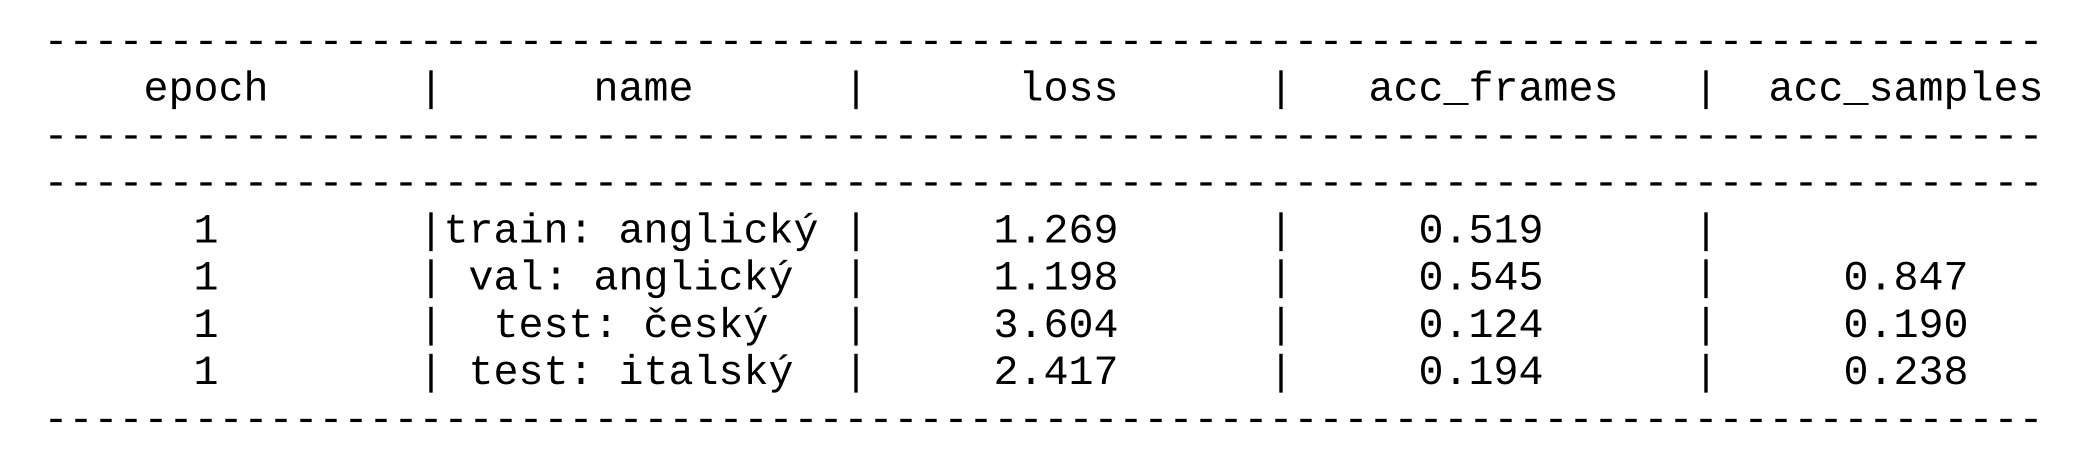
\includegraphics[scale=.215]{train_log.png}}
\caption{Přehledný výpis průběhu trénování}
\label{fig:print}
\end{figure}
\FloatBarrier

\begin{figure}[ht]
\centerline{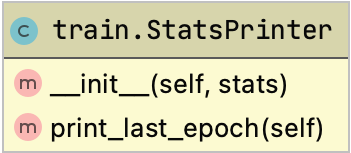
\includegraphics[scale=.32]{train-stats_printer.png}}
\caption{Třída StatsPrinter}
\label{fig:printer}
\end{figure}
\FloatBarrier

Po ukončení trénování lze model uložit do souboru s koncovkou .pt. Statistiky trénování lze uložit do souboru CSV. Ze statistik lze pomocí třídy Results (viz Obr. \ref{fig:results}) získat grafy průběhu trénování. Pomocí funkce plot z knihovny matplolib jsou vykresleny grafy průběhu trénování pro přesnosti a ztrátu. Dále jsou vytvořeny pomocí funkce heatmap z knihovny seaborn grafy matice záměn. Grafy lze zobrazit a uložit jako obrázky typu PNG.

\begin{figure}[ht]
\centerline{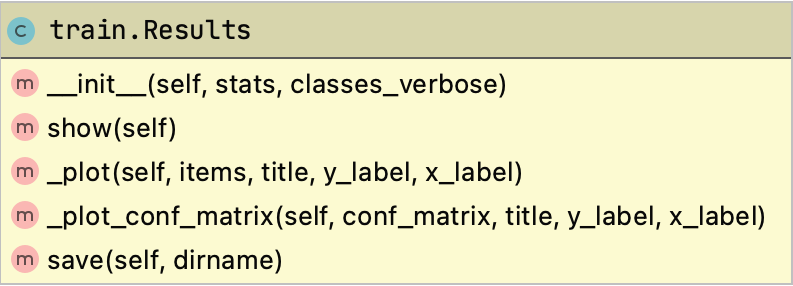
\includegraphics[scale=.3]{train-results.png}}
\caption{Třída Results}
\label{fig:results}
\end{figure}
\FloatBarrier

\chapter{Experimenty}
Bylo provedeno několik experimentů pro vyladění hyperparametrů modelu. Jako první byl proveden výchozí experiment. Trénovací, validační a testovací sady byly vytvořeny ze všech vybraných anglických datových sad a italské datové sady. Z každé vybrané datové sady byly rovnoměrně rozděleny vzorky podle tříd do sad v poměru 80 \% nahrávek přišlo do trénovací sady, 10 \% do sady testovací a 10 \% do sady validančí.

\section{Výchozí model}
Jako první byl vytvořen výchozí model, který slouží k porovnání výkonu mezi modely. Pro získání ztráty modelu byla jako kriteriální funkce zvolena křížová entropie. Byl zvolen algoritmus Adaptive Momentum (Adam) pro optimalizaci modelu a míra učení byla nastavena na hodnotu 0,001. Model se skládal ze tří skrytých lineárních vrstev o šířce 128 neuronů. Ve skryté vrstvě byla použita aktivační funkce ReLU. Model byl trénován 10 epoch s velikostí jedné dávky 256 vzorků. Velikost pravého a levého okolí byla rovna 25 vzorkům. Bylo klasifikováno 7 emocí: hněv, znechucení, strach, radost, překvapení, smutek a neutrální stav.

Během trénování modelu přesnost pro vzorky na trénovací sadě stoupala až k hodně 83,1 \% a na trénovací sadě kolísala kolem 59 \%. Ztráta modelu na trénovací sadě postupně klesala. U validační a testovací sady ztráta mírně stoupala. Přesnost pro nahrávky dosáhla kolem 87 \% na validační a testovací sadě. Úspěch dokládá i rozložení předpovědí v matici záměn, kde je většina předpovědí umístěna na hlavní diagonále.

\begin{figure}[!htbp]
\centerline{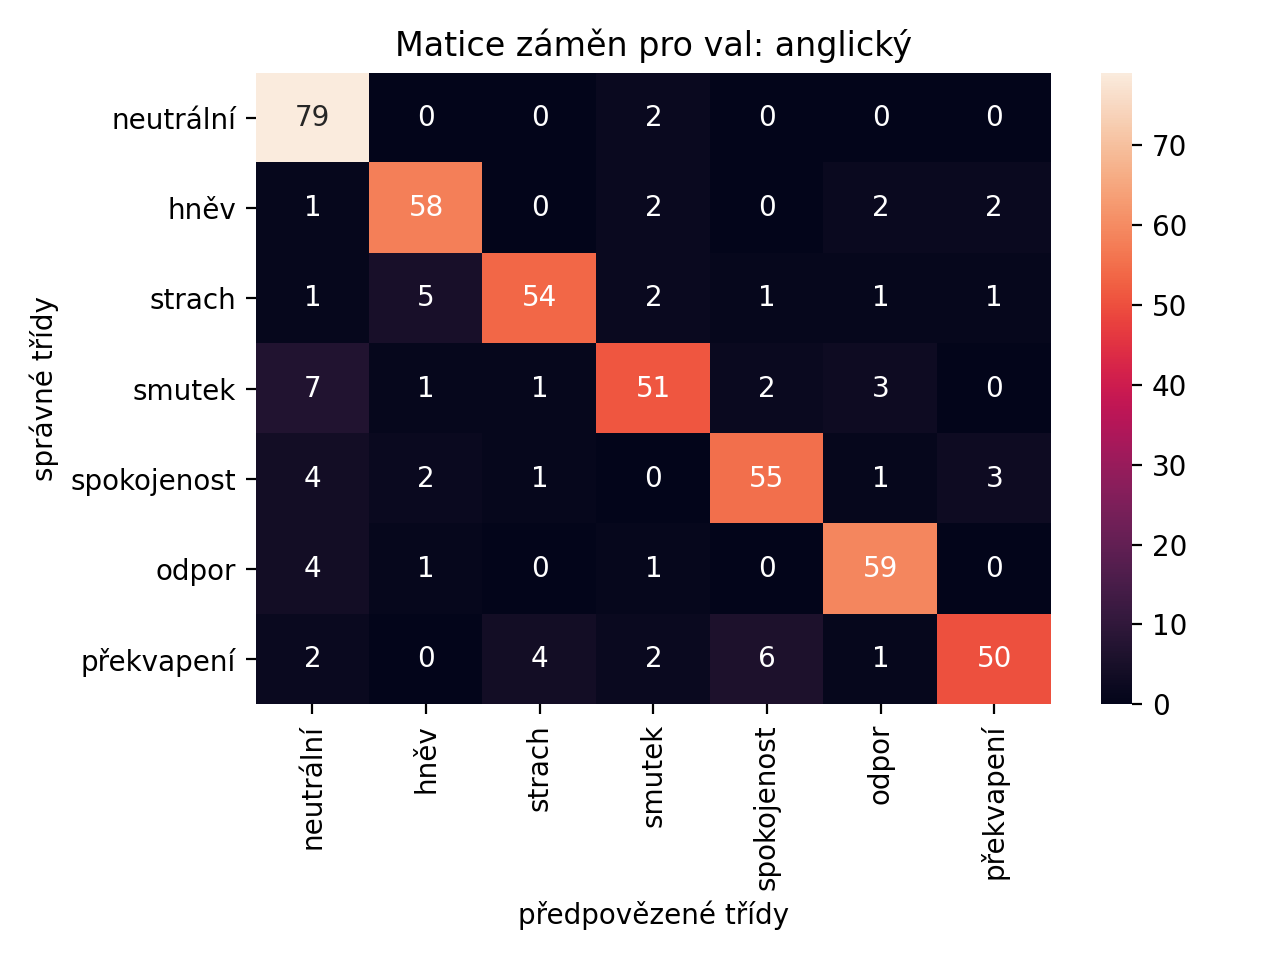
\includegraphics[scale=.5]{baseline-conf_matrix-val.png}}
\caption{Matice záměn pro validační sadu}
\label{fig}
\end{figure}
\FloatBarrier

\begin{figure}[!htbp]
\centerline{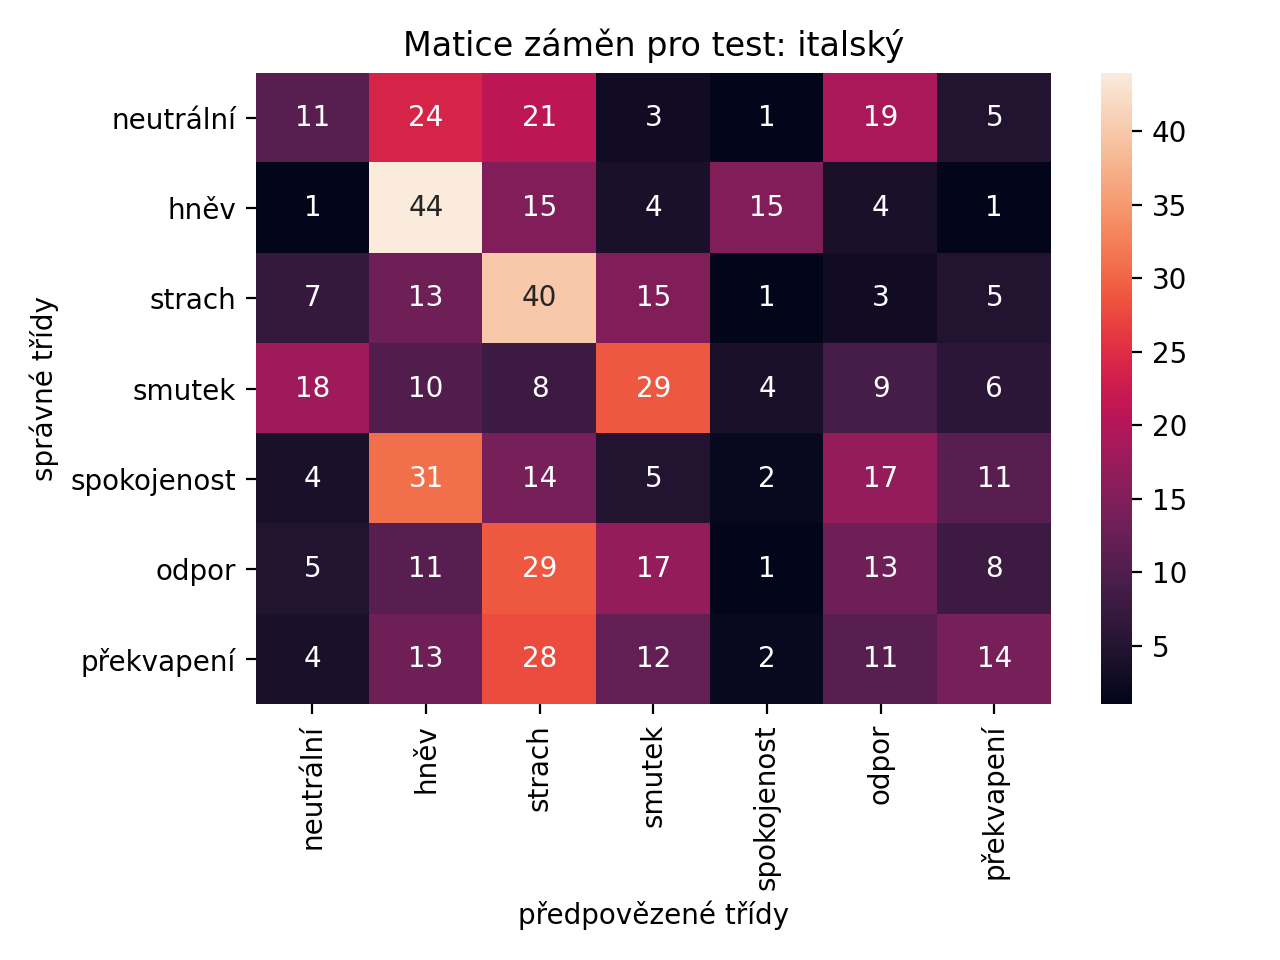
\includegraphics[scale=.5]{baseline-conf_matrix-test.png}}
\caption{Matice záměn pro testovací sadu}
\label{fig}
\end{figure}
\FloatBarrier

Následně bylo provedeno několik pokusů se snahou vyladit hyperparametry modelu. Byla měněna především architektura sítě, počet a šířka vrstev. Upravovány byly také velikosti okolí vzorku. Trénování probíhalo během 10 epoch, jelikož bylo zjištěno u výchozího pokusu, že tento počet postačí pro získání představy o výkonu modelu. Kriteriální a optimalizační funkce zůstali stejné.

\section{Změny počtu skrytých vrstev}
Byly provedeny tři experimenty, jejíž cílem bylo zjistit optimální počet skrytých vrstev modelu. Byly vyzkoušeny modely se dvěma, čtyřmi a pěti vrstvami. Tři vrstvy byly vynechány, jelikož je měl výchozí model. Z grafů pro trénovací data lze usoudit, že s rostoucím počtem vrstev stoupá i přesnost modelu a zároveň klesá ztráta. Přesnost pro vzorky na validační a testovací sadě také roste s počtem skrytých vrstev. Nicméně s ní vrůstá i ztráta, která by měla naopak klesat. Průběh ztráty u modelů se třemi a více vrstvami se příliš nemění. Při počtu dvou vrstev se model učí pomaleji, ale zároveň neroste v takové míře ztráta.

\begin{figure}[!htbp]
\centerline{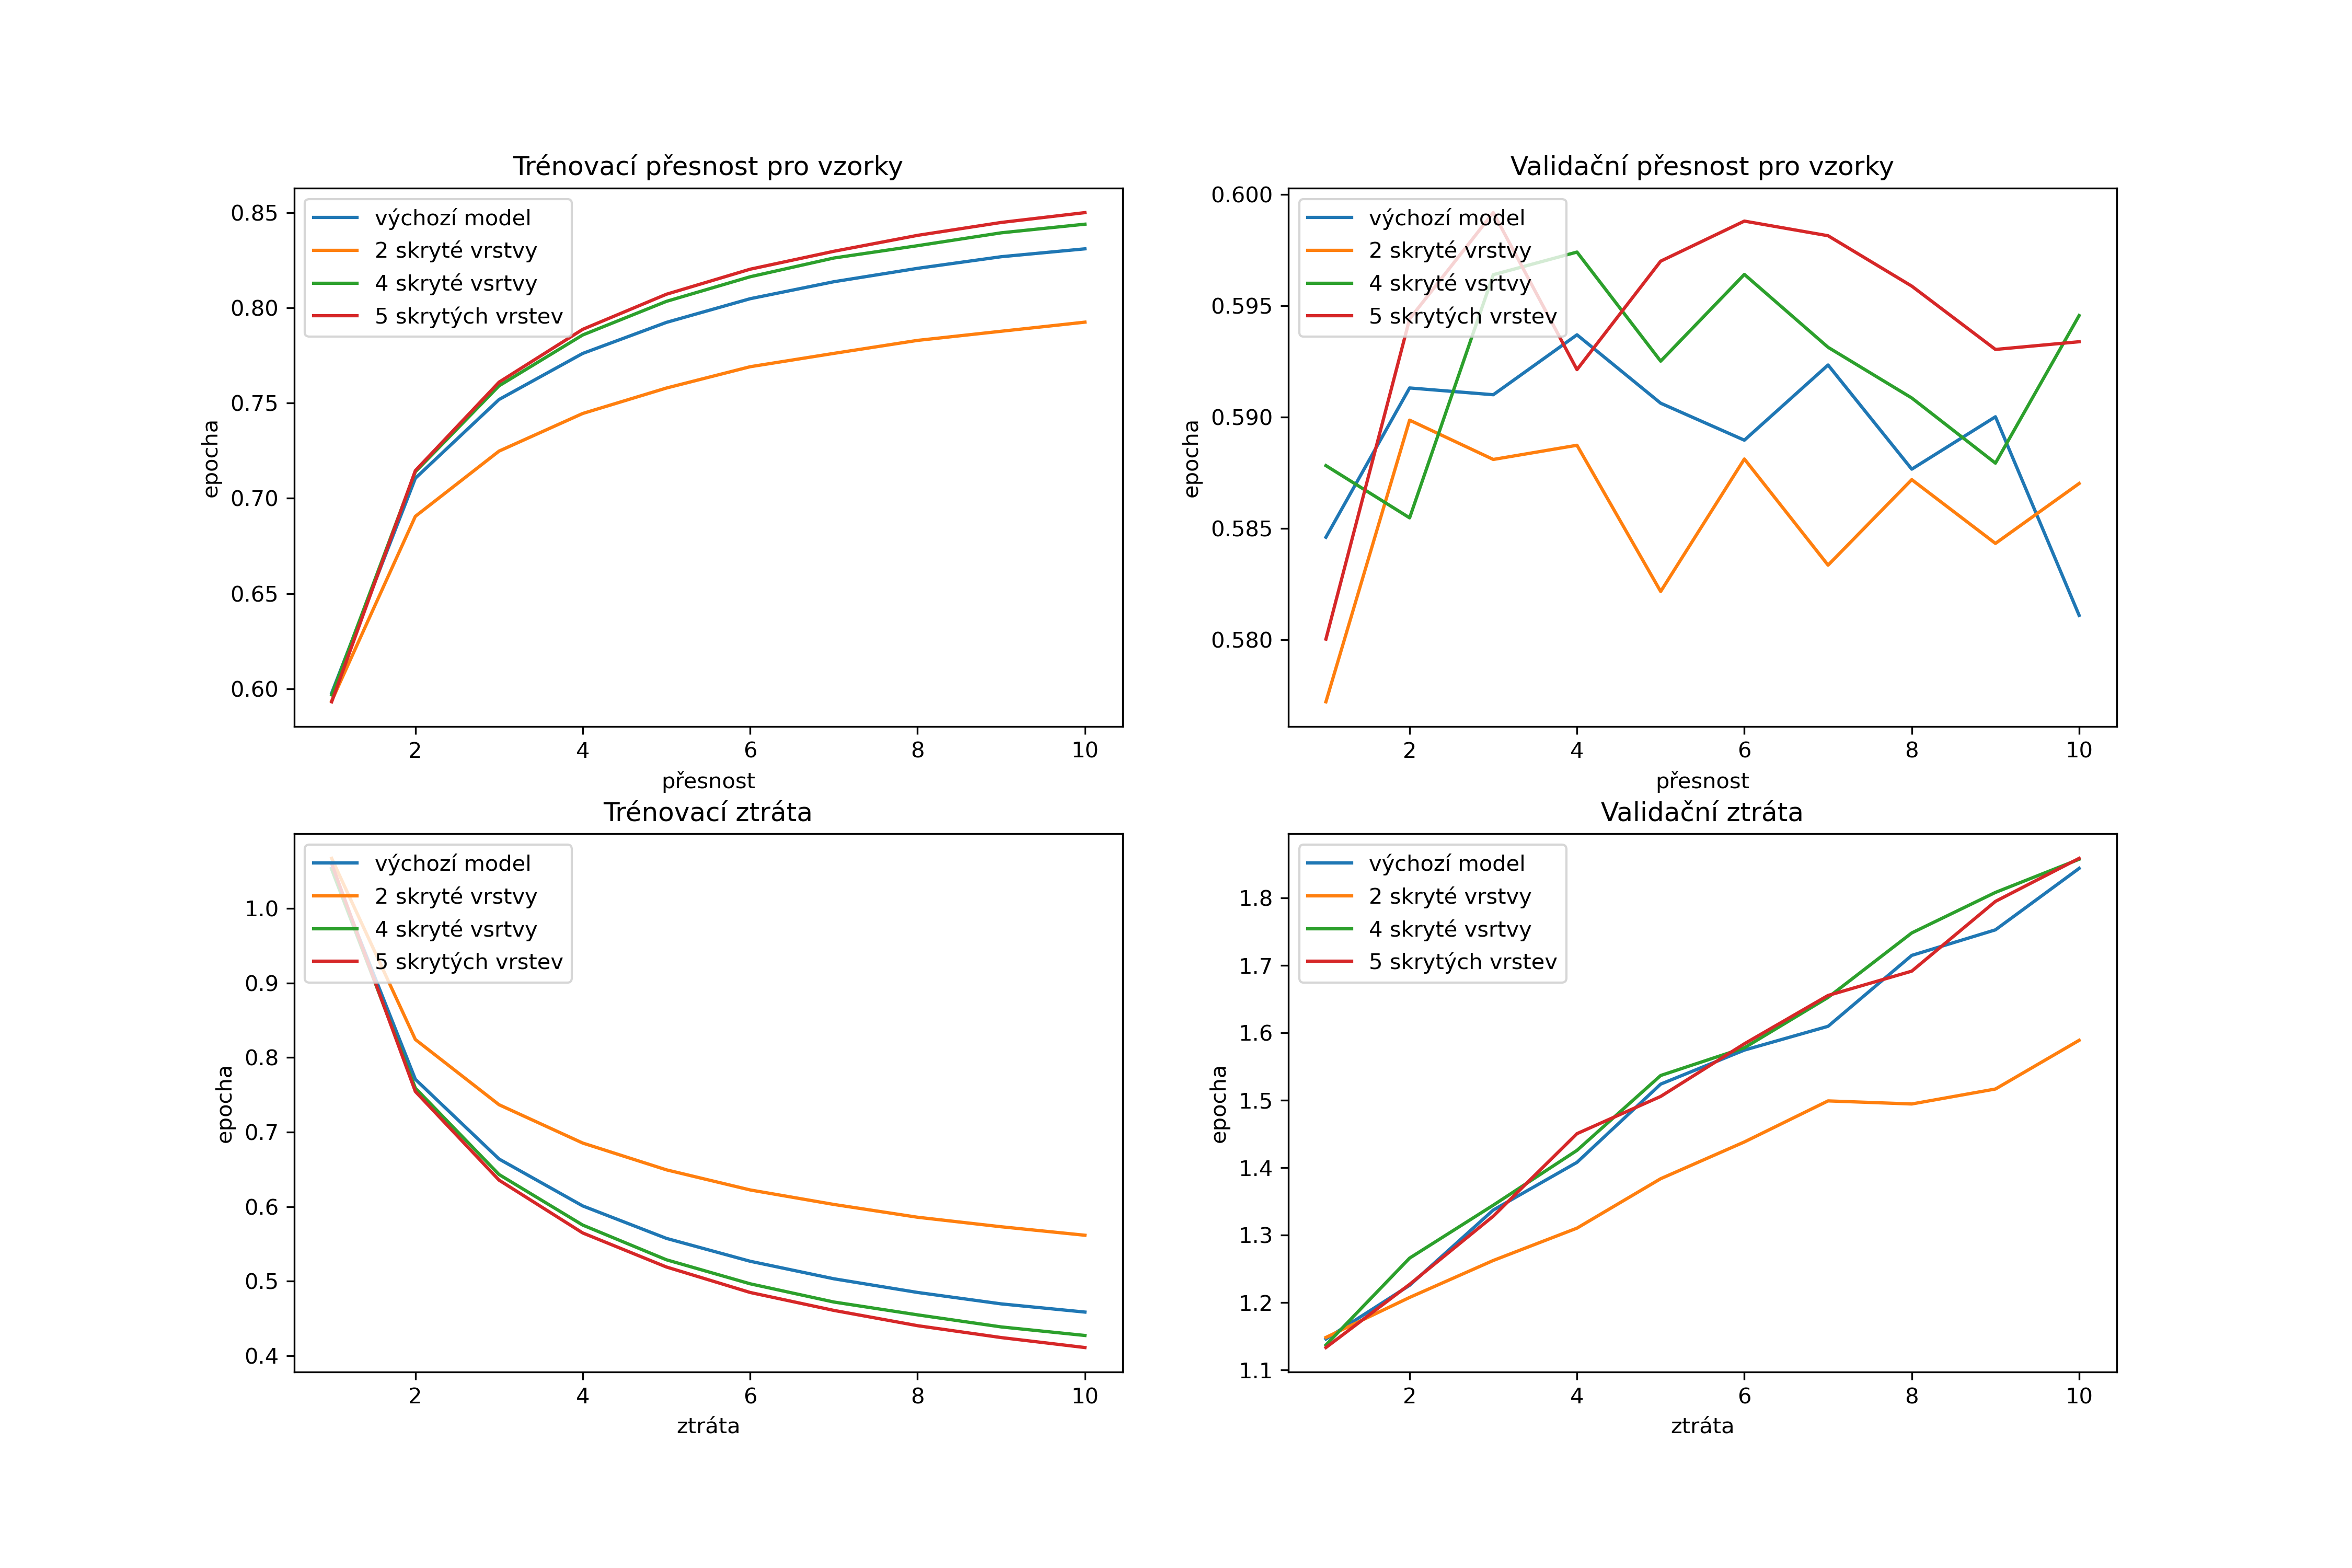
\includegraphics[scale=.5]{training_course-layers.png}}
\caption{Přehled průběhu trénování}
\label{fig}
\end{figure}
\FloatBarrier

\section{Změny velikosti okolí vzorku}
Velikost okolí vzorku bylo možné také upravovat. Celkem byly provedeny 4 pokusy, při nichž velikost okolí pro pravou a levou stranu nabývala hodnot 5, 10, 30 a 50. Z průběhu grafů pro trénovací datovou sadu lze usoudit, že se zvyšujícím se okolí stoupá i přesnost a klesá ztráta modelu. U validační a testovací sady přesnost pro vzorky stoupá stejným způsobem jenom pomaleji. Zároveň však stoupá ztráta modelu.

\begin{figure}[!htbp]
\centerline{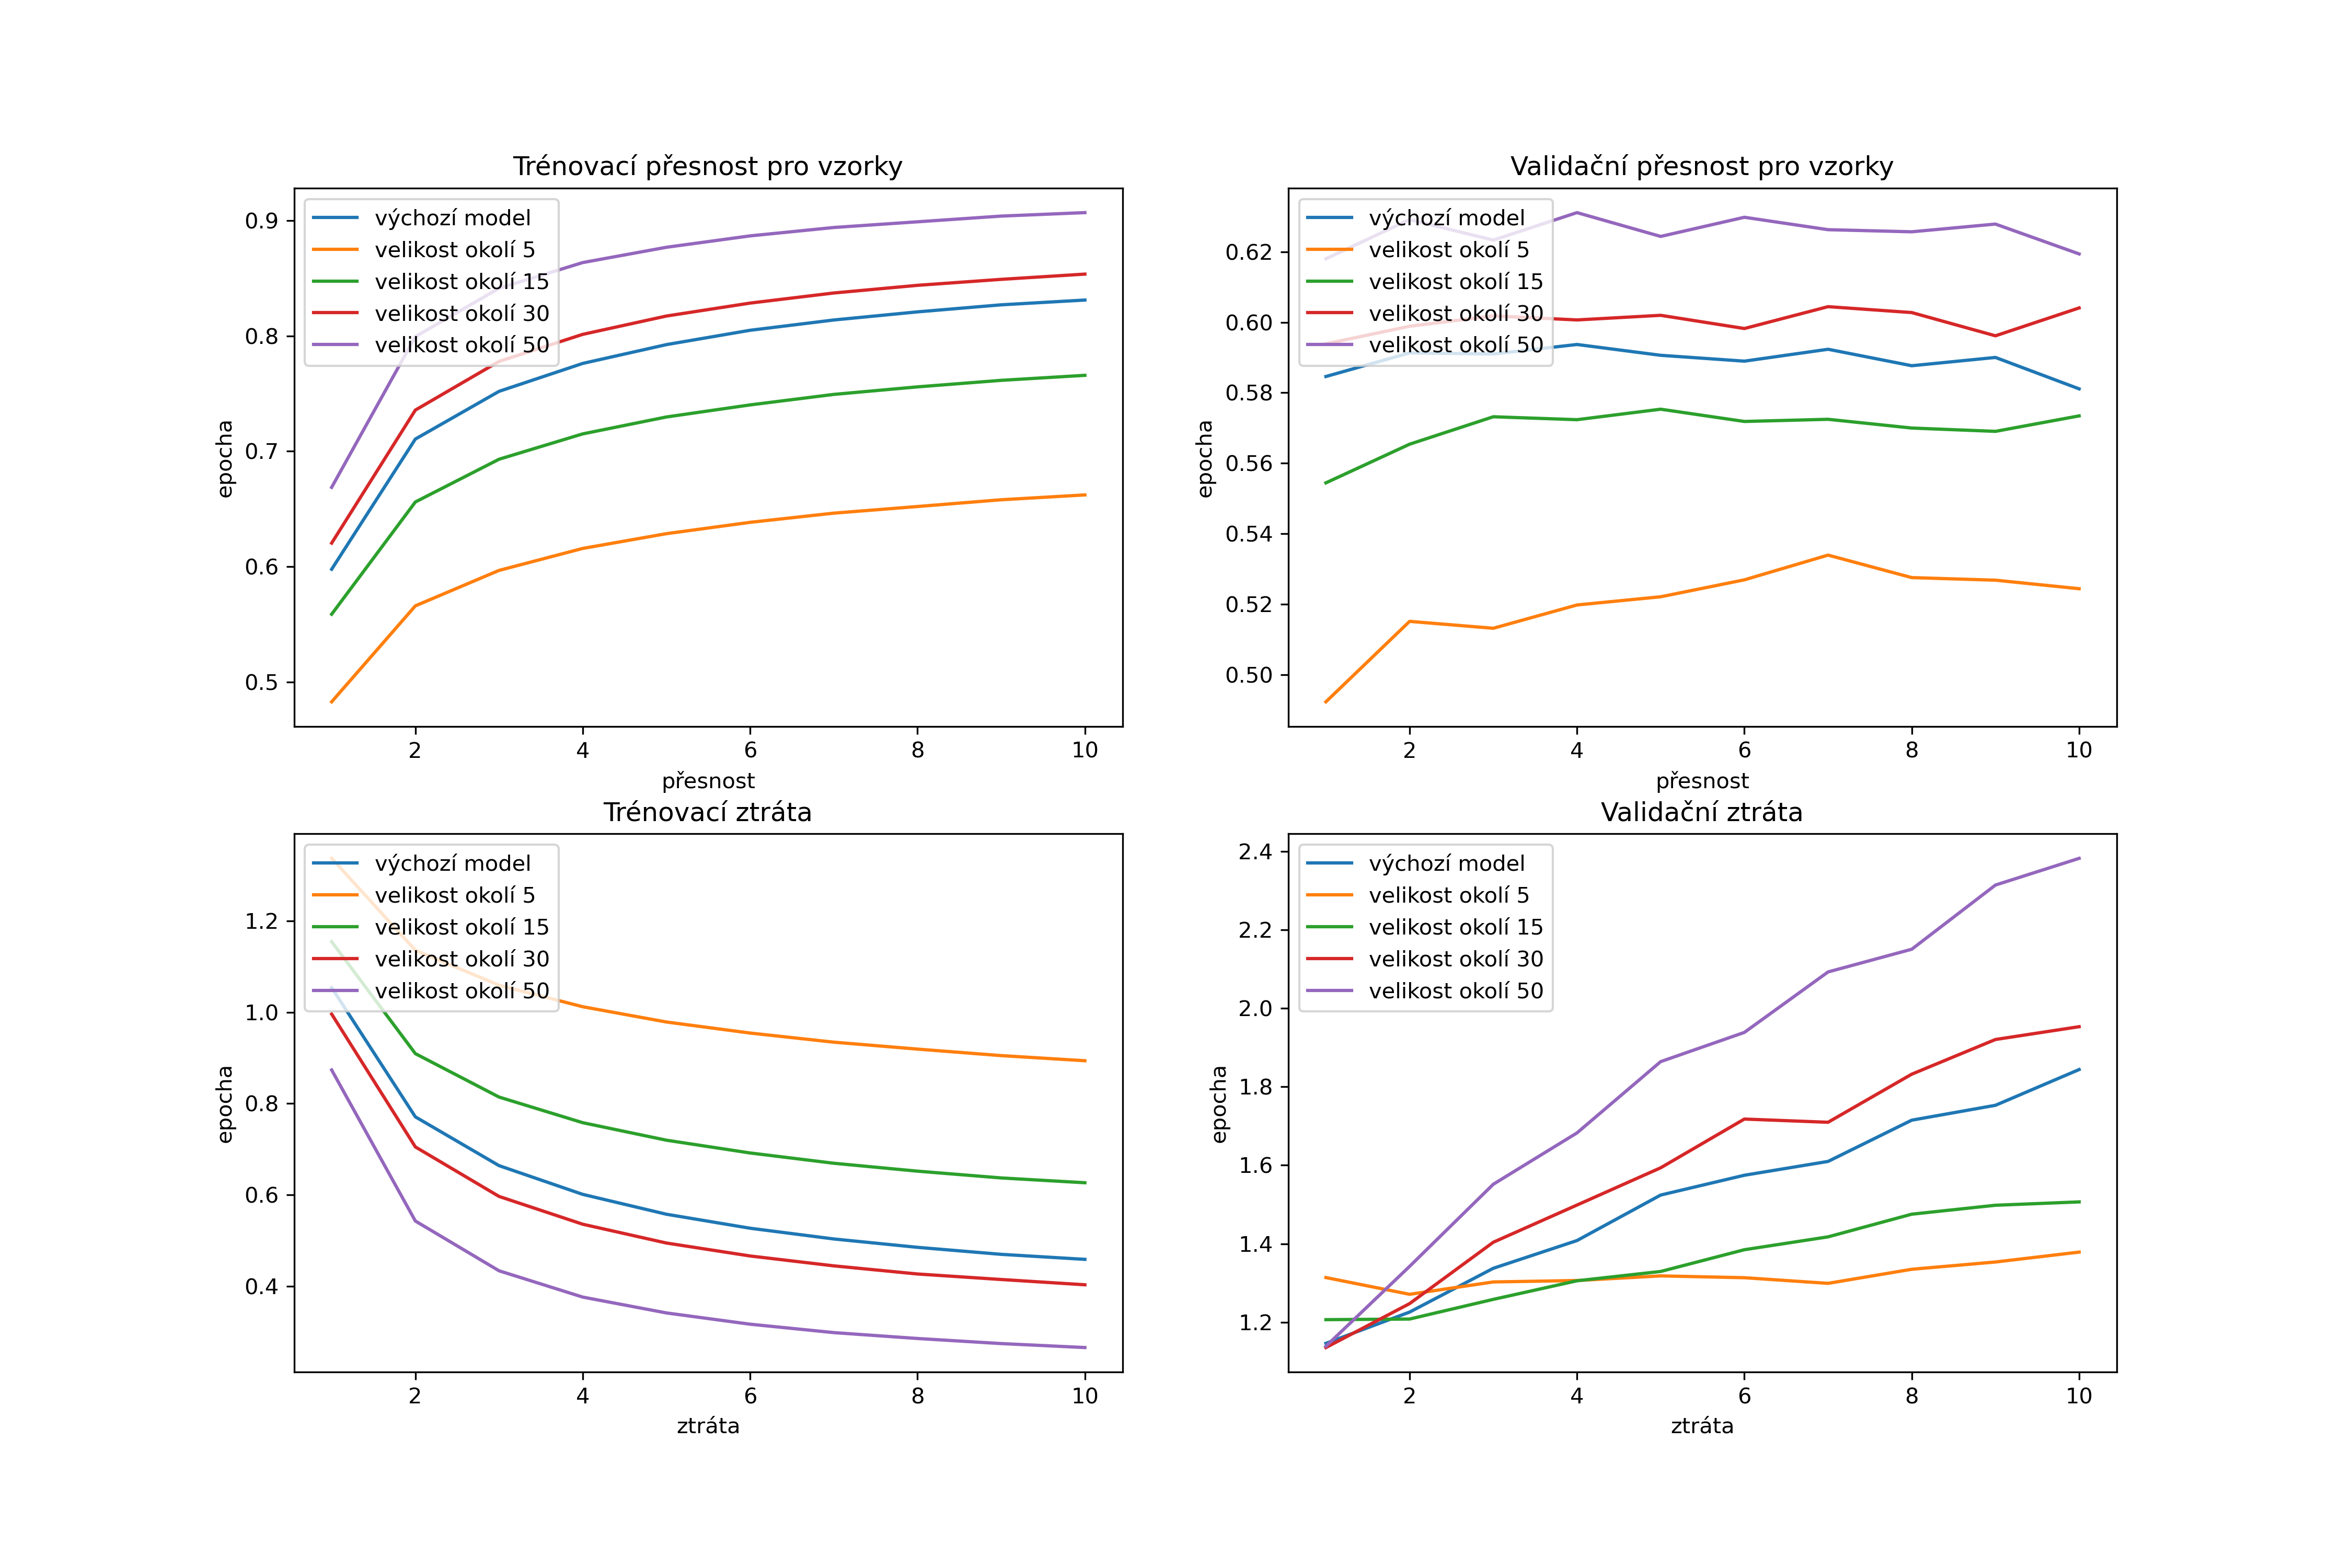
\includegraphics[scale=.5]{training_course-margin.png}}
\caption{Přehled průběhu trénování}
\label{fig}
\end{figure}
\FloatBarrier

\section{Změny šířky skrytých vrstev}
Další parametr, který lze měnit, je šířka skrytých vrstev modelu. Uskutečnily se 4 experimenty, během kterých nabývala šířka vrstev hodnot od 16 do 512 neuronů. Při srovnání přesností pro trénovací datovou sadu si lze všimnout, že model s 16 neurony dosahuje nejnižší přesnosti kolem 50 \%. Dále s přibývající šířkou výsledná přesnost stoupá přibližně o 10 \%, kromě modelu s šířkou 256 a 512, kde je rozdíl mezi přesností podstatně menší.  Na grafu ztráty pro validační sadu lze vidět, že ztráta klesá pro model se šířkou 16 neuronů. Pro model se šířkou 64 neuronů je ztráta téměř konstantní a pro modely se šířkou 256 a 512 výrazně stoupá. Vzhledem k tomu, že modely s vyšším počtem neuronů mají tendenci se přeučovat zvolil bych model s šířkou mezi 64 a 128 neurony.

\begin{figure}[!htbp]
\centerline{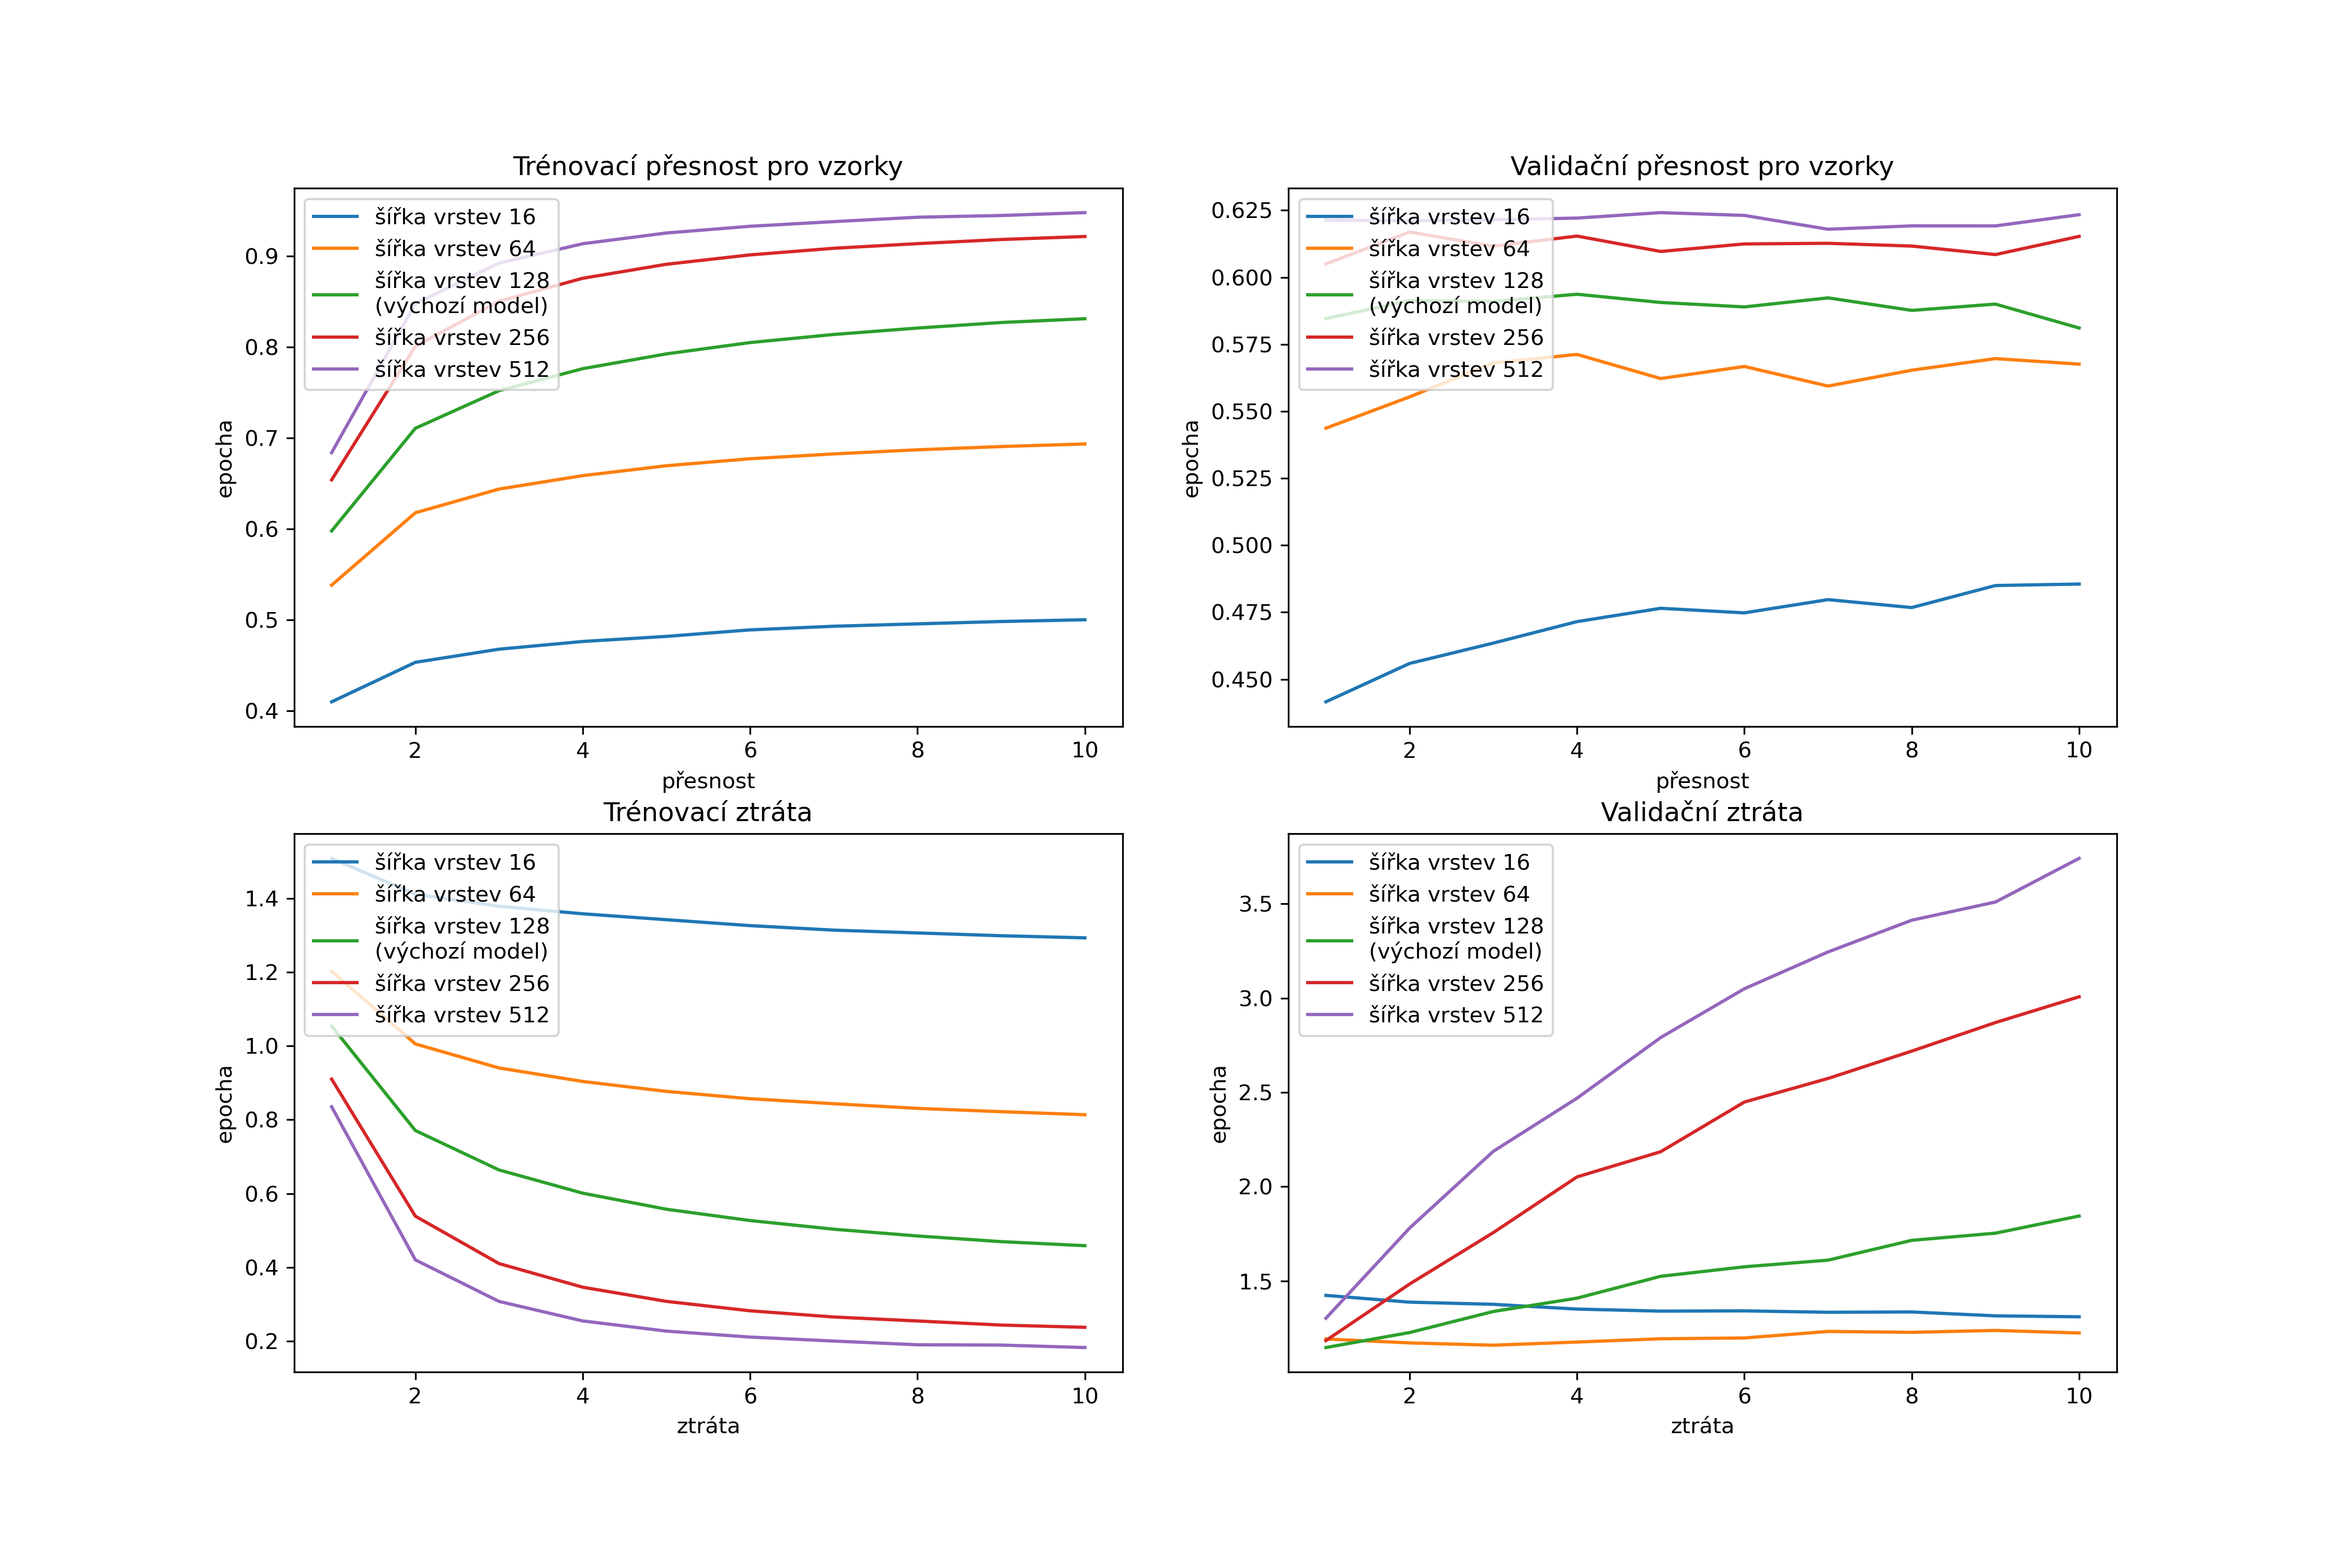
\includegraphics[scale=.5]{training_course-width.png}}
\caption{Přehled průběhu trénování}
\label{fig}
\end{figure}
\FloatBarrier

\section{Omezení počtu emocí}
V další řadě experimentů byly měněny počty emocí. Při experimentu se čtyřmi emocemi byly sjednoceny emoce hněvu a odporu na hněv, překvapení a spokojenost na spokojenost, smutek a strach na smutek. Se třemi emocemi byly rozlišovány pouze neutrální stav, negativní a pozitivní emoce. Mezi pozitivní emoce patřila spokojenost s překvapením a mezi negativní emoce hněv, odpor, smutek a strach. Z grafů pro trénovací sadu lze usoudit, že s menším počtem emocí stoupá přesnost a zároveň klesá ztráta modelu. V grafech pro validační sadu lze zpozorovat, že přesnost pro vzorky s ubývajícím počtem emocí roste, ale její průběh je konstantní. Ztráta u jednotlivých modelů lineárně roste.

\begin{figure}[!htbp]
\centerline{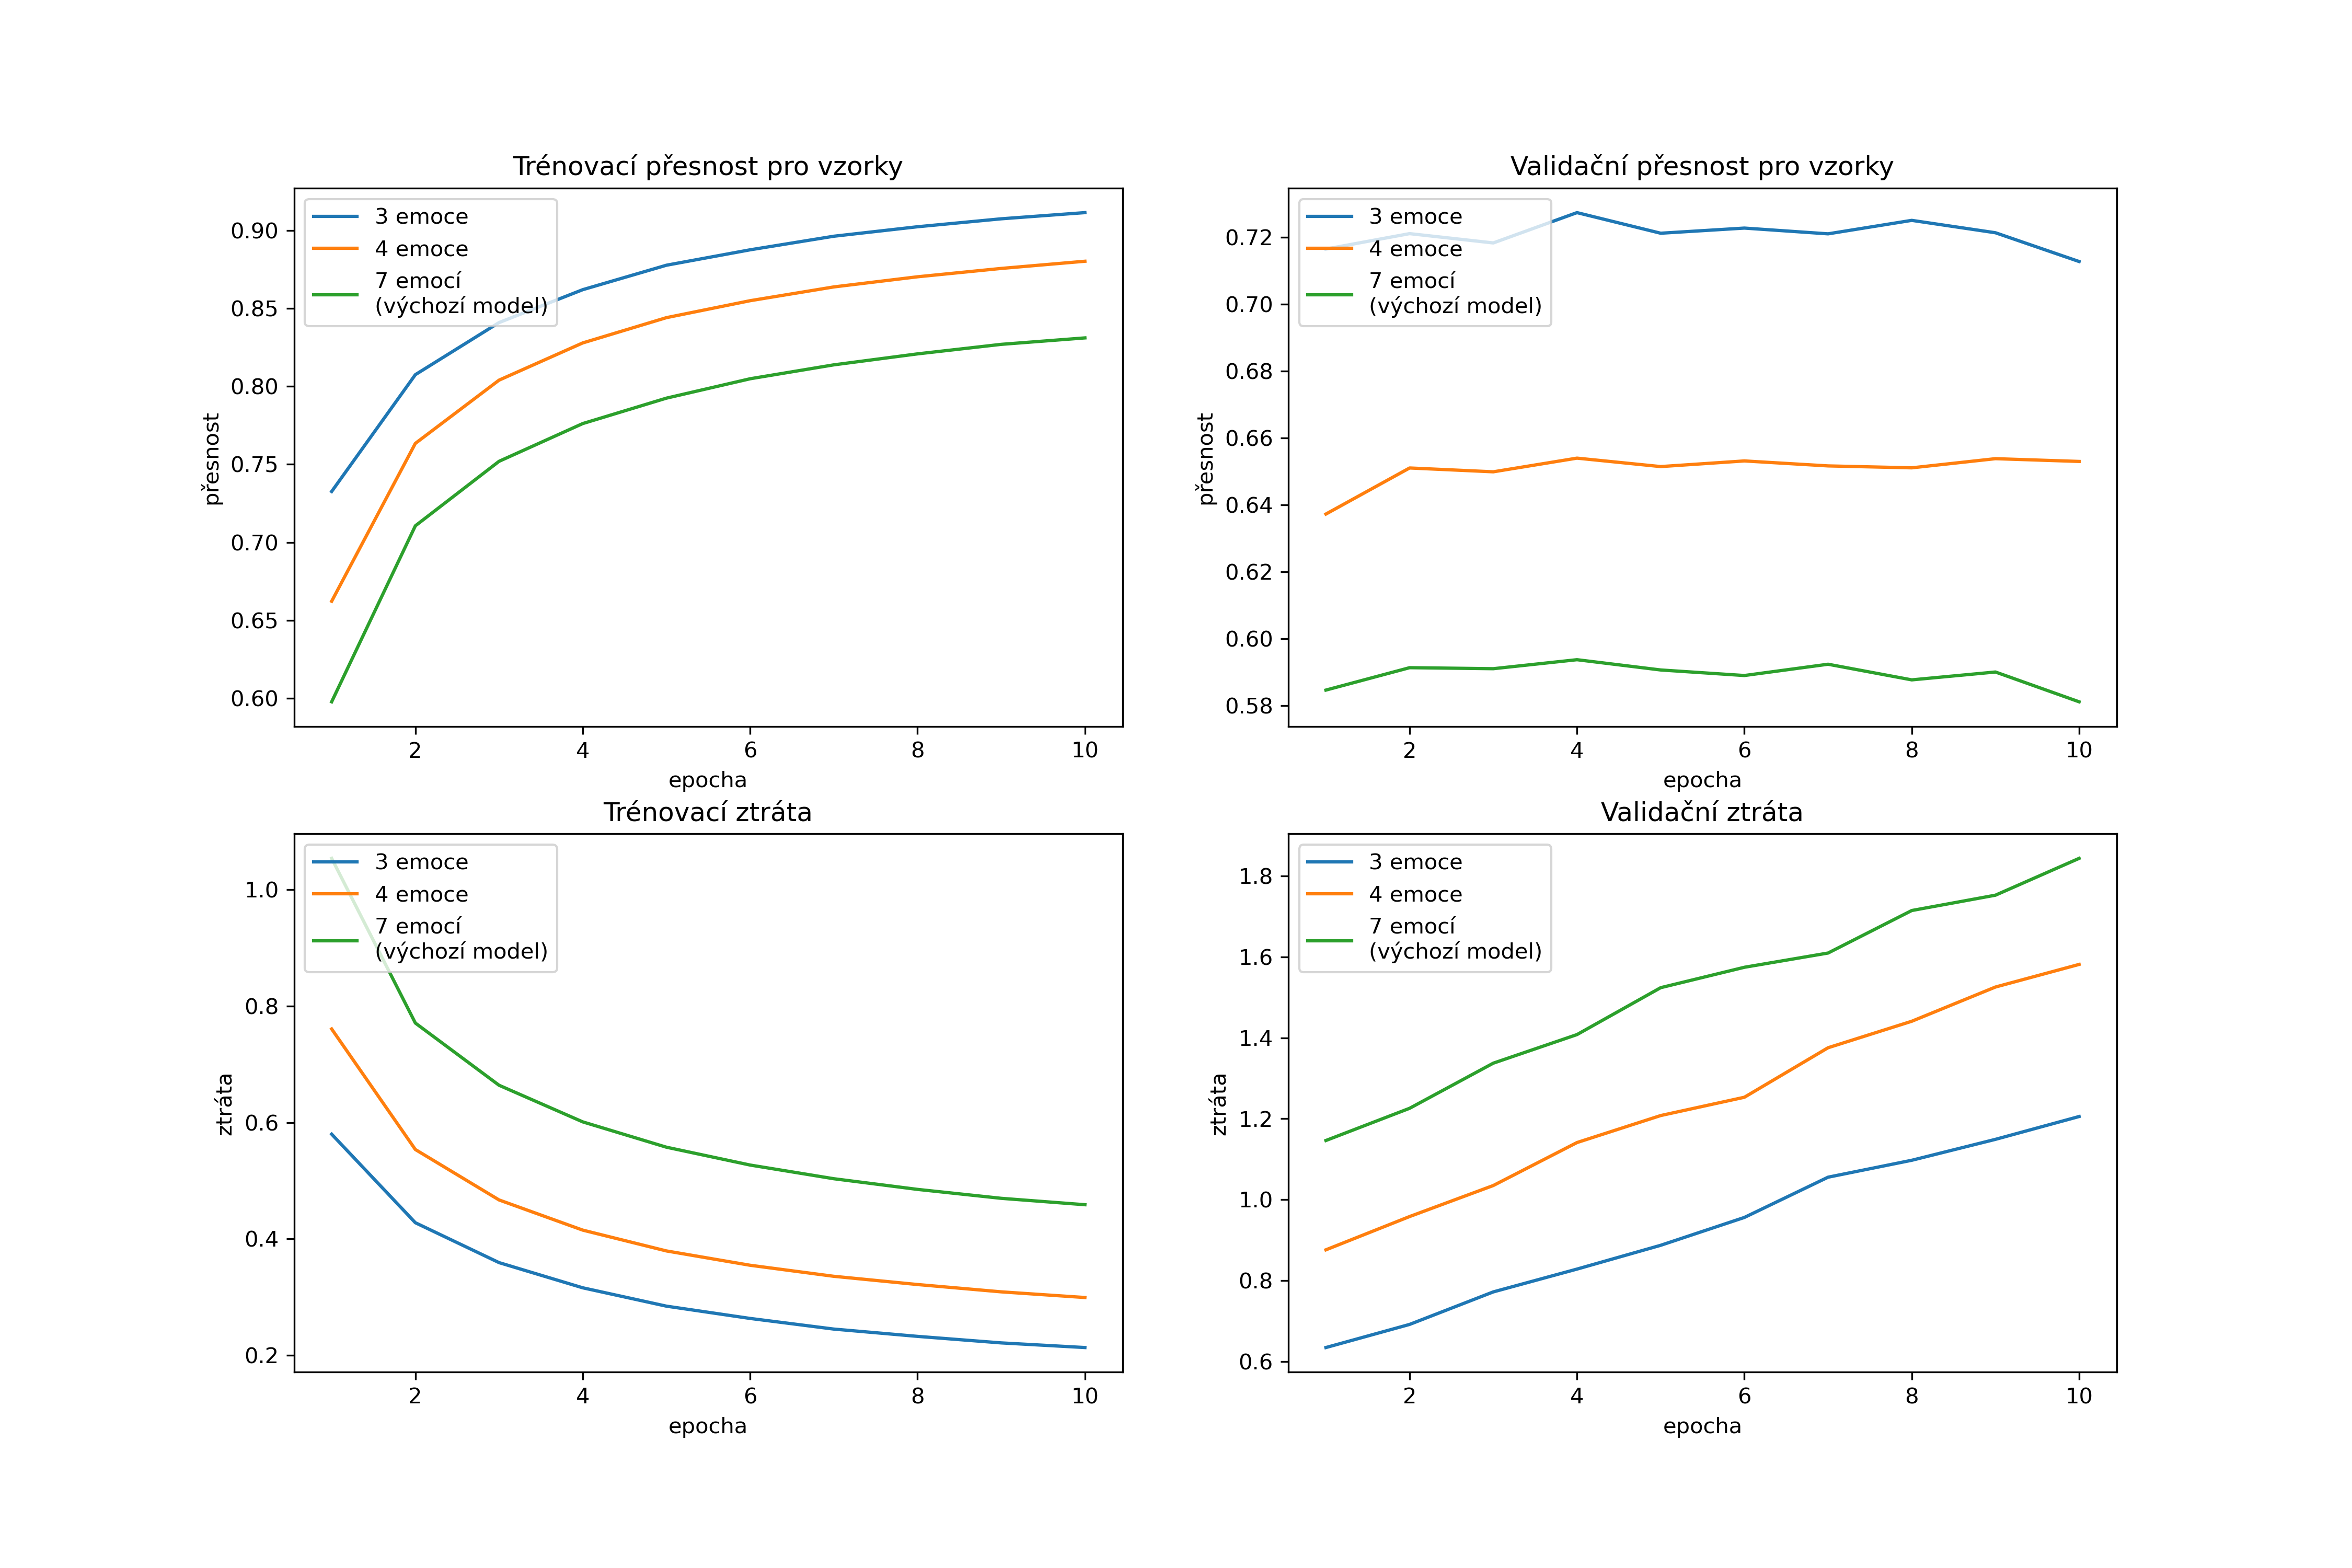
\includegraphics[scale=.5]{training_course-emotion_reduction.png}}
\caption{Přehled průběhu trénování}
\label{fig}
\end{figure}
\FloatBarrier

Počet nahrávek pro jednotlivé třídy je mnohem vyrovnanější při klasifikaci do čtyřech tříd oproti klasifikaci do tří tříd. Při sloučení tříd pro klasifikaci do tří tříd byla největší část nahrávek umístěna do negativní třídy (viz Obr. \ref{fig:3_emotions-conf_matrix-val}). 

\begin{figure}[!htbp]
\centerline{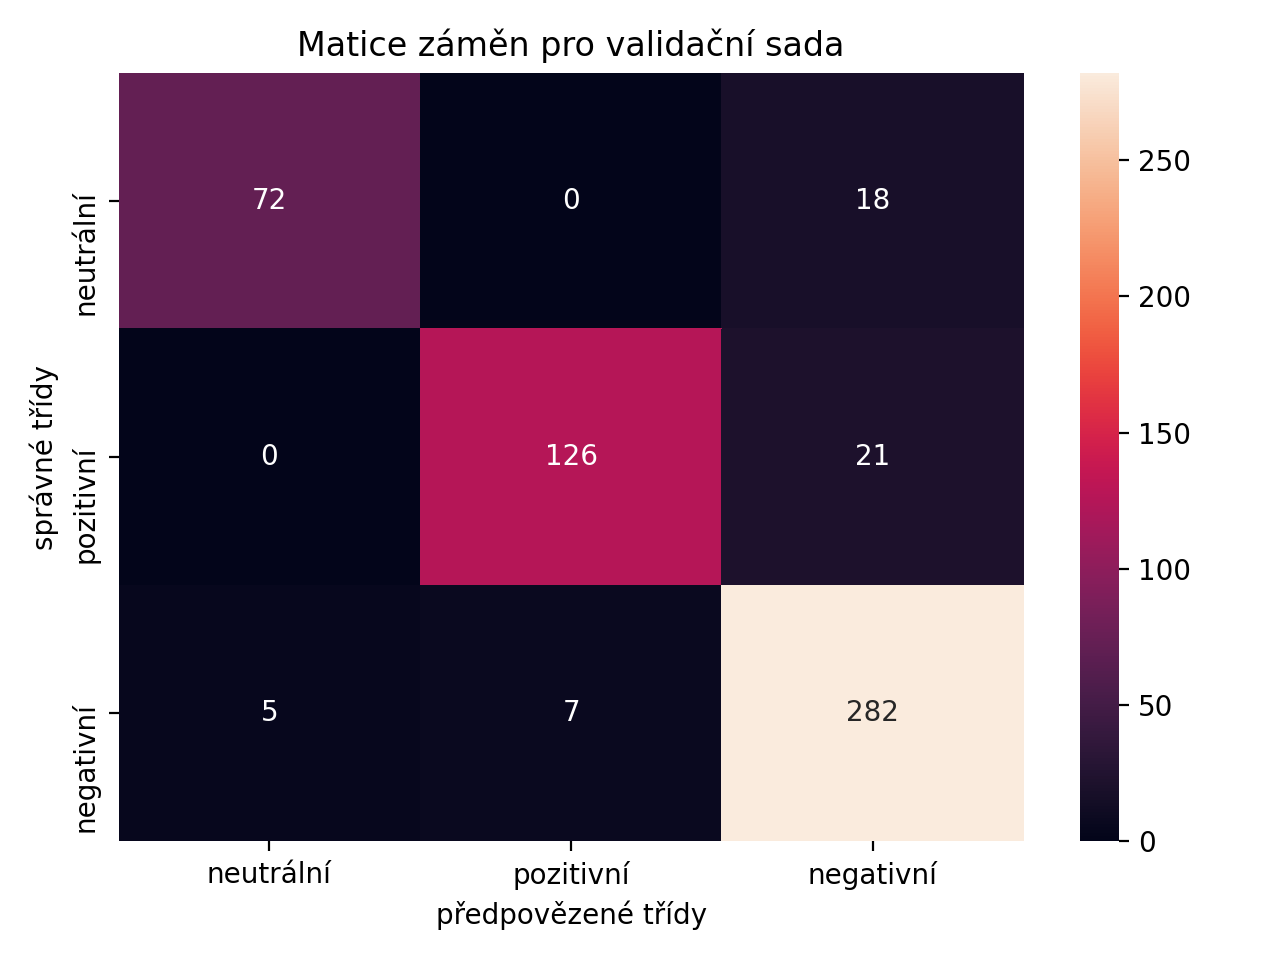
\includegraphics[scale=.5]{3_emotions-conf_matrix-val.png}}
\caption{Matice záměn pro validační data ke klasifikaci 3 emocí}
\label{fig:3_emotions-conf_matrix-val}
\end{figure}
\FloatBarrier

Při klasifikaci do čtyřech tříd byly nahrávky rozděleny téměř rovnoměrně do tříd hněvu, spokojenosti a smutku (viz Obr. \ref{fig:4_emotions-conf_matrix-val}). O trochu méně nahrávek bylo umístěno v neutrální třídě.

\begin{figure}[!htbp]
\centerline{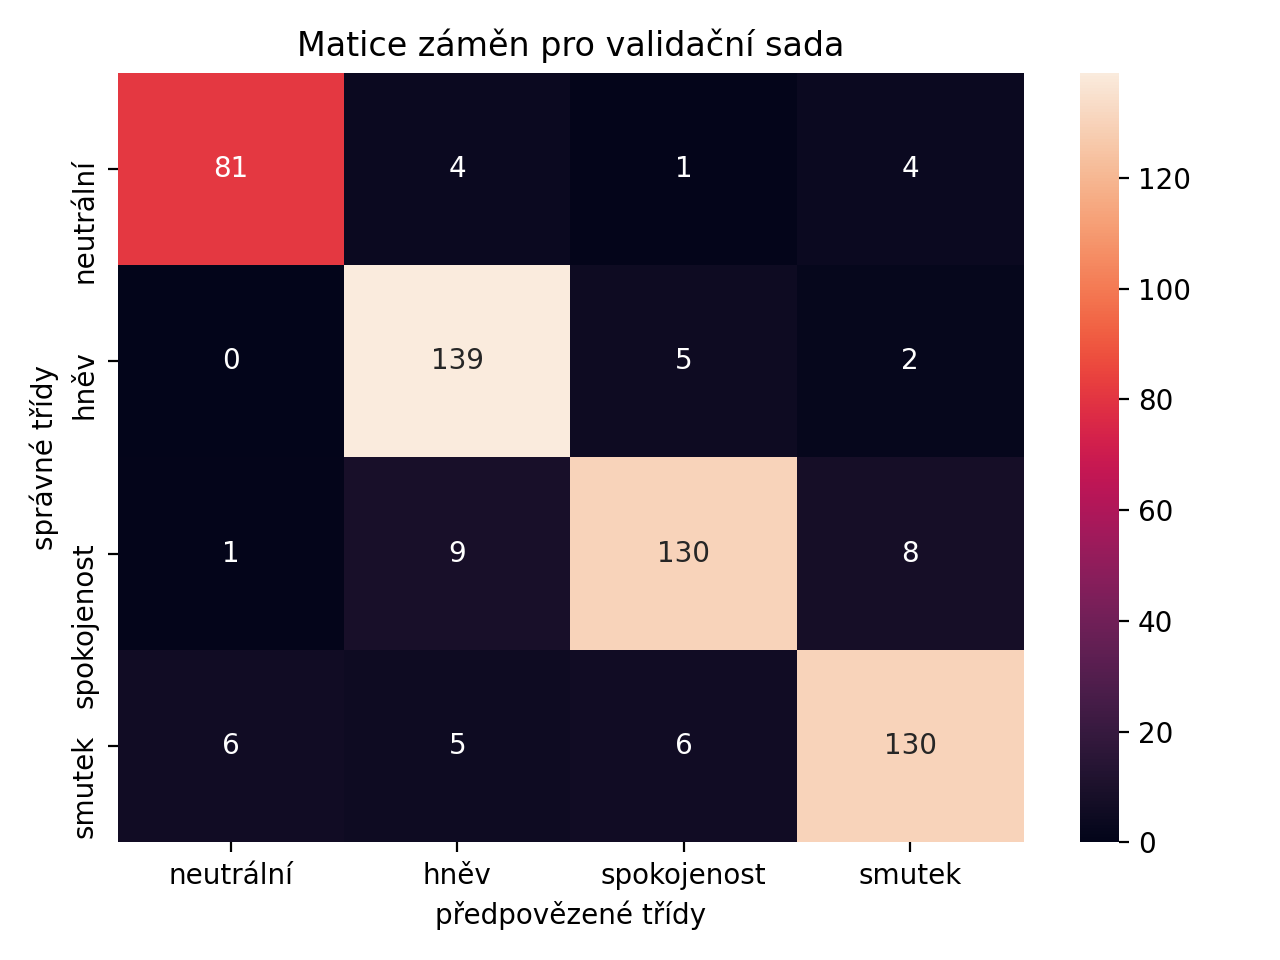
\includegraphics[scale=.5]{4_emotions-conf_matrix-val.png}}
\caption{Matice záměn pro validační data ke klasifikaci 4 emocí}
\label{fig:4_emotions-conf_matrix-val}
\end{figure}
\FloatBarrier

\section{Použití regularizace}
Jelikož u předchozích experimentů docházelo přeučování na testovací a validační sadě, bylo vyzkoušeno několik způsobů regularizace s cílem zamezení přeučování.

\begin{figure}[!htbp]
\centerline{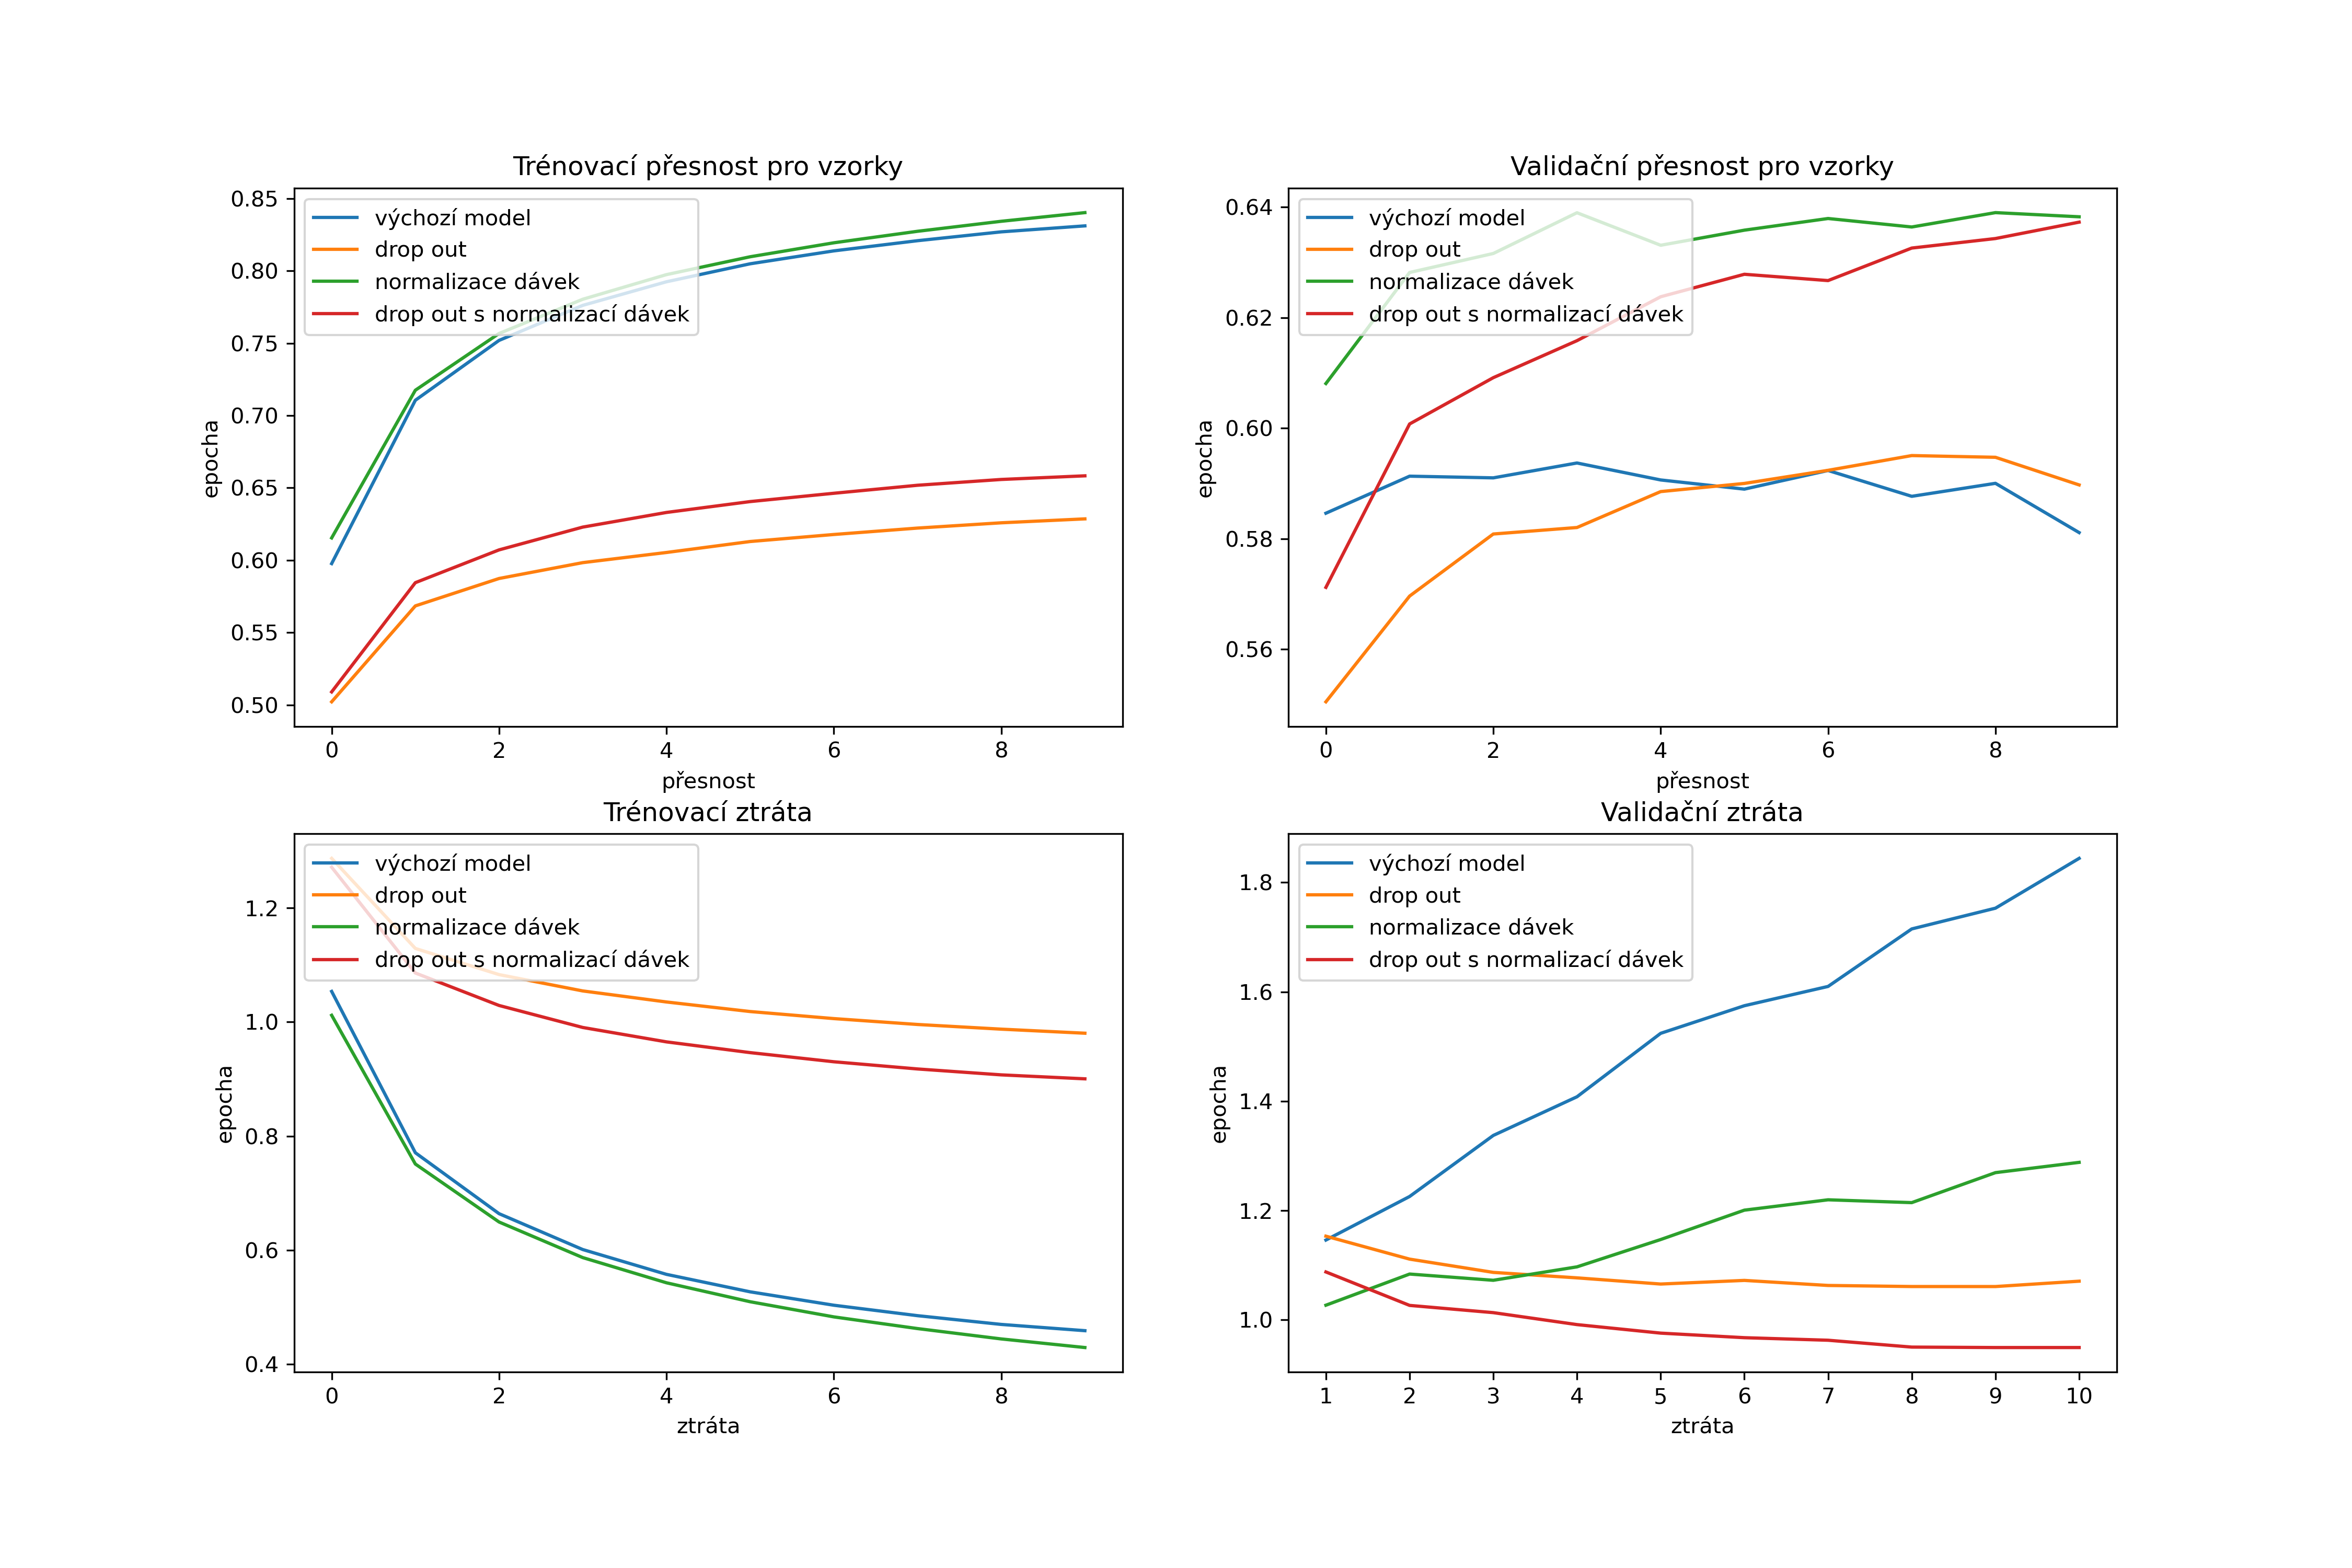
\includegraphics[scale=.5]{training_course-regularization.png}}
\caption{Přehled průběhu trénování}
\label{fig}
\end{figure}
\FloatBarrier

U prvního experimentu byly přidány za aktivační funkce ve skryté vrstvě drop out vrstvy s pravděpodobností 50 \%, že se výstup vynuluje. Tento model dosahoval nižší přesnosti pro vzorek na trénovacích datech než výchozí model a ztráta klesala pomaleji. Nicméně na validačních datech měla přesnost pro vzorky tendenci růst a dosáhla lepší přesnosti než výchozí model. Z grafu pro ztrátu je také vidět, že ztráta v průběhu trénování klesala. 

Pro další pokus byly skryté vrstvy výchozího modelu rozšířeny o vrstvy s normalizací dávek. Normalizace byly opět umístěny za aktivační funkce. Model dosahoval velice podobných výsledků ztráty a přesnosti na trénovacích datech. Nicméně průběhy trénovaní na validační sadě byly různé. Přesnost modelu dosáhla o 5 \% více než na výchozím modelu a po celou dobu trénování rostla. Míra růstu ztráty byla podstatně nižší. 

U posledního experimentu byla použita kombinace předchozích technik. Za aktivační funkci byla nejdříve umístěna normalizace dávek následovaná drop out vrstvou. Model dosáhl zatím nejlepších výsledků. Průběhy ztráty a přesnosti byly o trochu lepší než u modelu jenom s drop out vrstvami. Avšak přesnost pro vzorky na validanční sadě stoupala rychleji a dosahla stejných konečných výsledků jako model jenom s normalizacemi. Ztráta klesala více než u modelu s drop out vrstvami.

Na základě těchto výsledků jsem se pro další pokusy rozhodl použít model s normalizací dávek a drop out vrstvami.

\section{Finální modely}
Jako poslední byly vytvořeny finální modely pro klasifikaci do tří, čtyř a sedmi tříd. Byly použity různé modifikace modelu s normalizací dávek a drop out vrstvami ve skryté vrstvě. Pro všechny počty emocí byly vyzkoušeny tři modely. Průběhy trénování jsou vykresleny v přehledu \ref{fig:final_training_course}.

První model měl tři skryté vrstvy o šířce 64 neuronů a vzorek do sítě vstupoval s velikostí 30 pravého a levého okolí. Tento typ architektury se osvědčil při klasifikaci do tří tříd. Během 26. epochy došlo k získání nejlepších výsledků, kdy model dosáhl přesnosti pro vzorky 77,4 \% na trénovací sadě, 73,4 \% na validančí sadě a 75,4 \% na testovací sadě. Byla získána přesnost pro nahrávky 83,2 \% na validační sadě a 84,7 \% na sadě testovací.

Další model se skládal ze tří skrytých vrstev o šířce 128 neuronů s velikostí 30 pravého a levého okolí. Při klasifikaci do čtyř a sedmi tříd model vykazoval dobré výsledky, které byly překonány posledním modelem.

Model, který se nejvíce osvědčil při klasifikaci do čtyř a sedmi tříd, se skládal ze čtyř s krytých vrstev o šířce 128 neuronů a vzorek do sítě vstupoval s velikostí 50 pravého a levého okolí. Při klasifikaci do čtyř tříd měl průběh trénování větší růst u přesnosti pro vzorky a větší spád ztráty než u předchozího modelu. Nicméně měl větší tendenci se přeučovat a nejlepších výsledků dosáhl na 10 epoše, kdy byly přesnosti pro vzorky na trénovací sadě 79 \%, validační sadě 73,7 \% a na testovací sadě 73,6 \%. Přesnost pro nahrávky vystoupala u validační sady na 91,7 \% a u testovací sady na 92,3 \%. Model dosáhl lepších výsledků přesnosti pro nahrávky než při klasifikaci do tří tříd pravděpodobně, kvůli rovnoměrnějšímu rozložení nahrávek do jednotlivých tříd. Při klasifikaci do sedmi tříd bylo dosaženo nejlepších výsledků v poslední epoše trénování. Přesnost pro vzorky vystoupala na trénovací sadě na 75,8 \%, na sadě validační na 69,3 \% a na testovací sadě 68 \%. Bylo dosaženo přesnosti pro nahrávky 90,4 \% na sadě validanční a 88,5 \% na sadě testovací.

\begin{table}
\centering
\resizebox{\textwidth}{!}{\begin{tabular}{|l|l|l|l|l|l|} 
\hline
\multicolumn{1}{|c|}{\multirow{2}{*}{počet tříd}} & \multicolumn{1}{c|}{trénovací sada} & \multicolumn{2}{c|}{validační sad} & \multicolumn{2}{c|}{testovací sada} \\ 
\cline{2-6}
\multicolumn{1}{|c|}{} & \multicolumn{1}{c|}{přesnost pro vzorek} & \multicolumn{1}{c|}{přesnost pro vzorek} & \multicolumn{1}{c|}{přesnost pro nahrávku} & \multicolumn{1}{c|}{přesnost pro vzorek} & \multicolumn{1}{c|}{přesnost pro nahrávku} \\ 
\hline
3 & 77,4 \% & 73,4 \% & 83,2 \% & 75,4 \% & 84,7 \% \\ 
\hline
4 & 79 \% & 73,7 \% & 91,7 \% & 73,6 \% & 92,3 \% \\ 
\hline
7 & 75,8 \% & 69,3 \% & 90,4 \% & 68 \% & 88,5 \% \\
\hline
\end{tabular}}
\caption{Přehled nejlepších výsledků finálních modelů}
\label{tab:best_results}
\end{table}
\FloatBarrier

\begin{figure}[!htbp]
\centerline{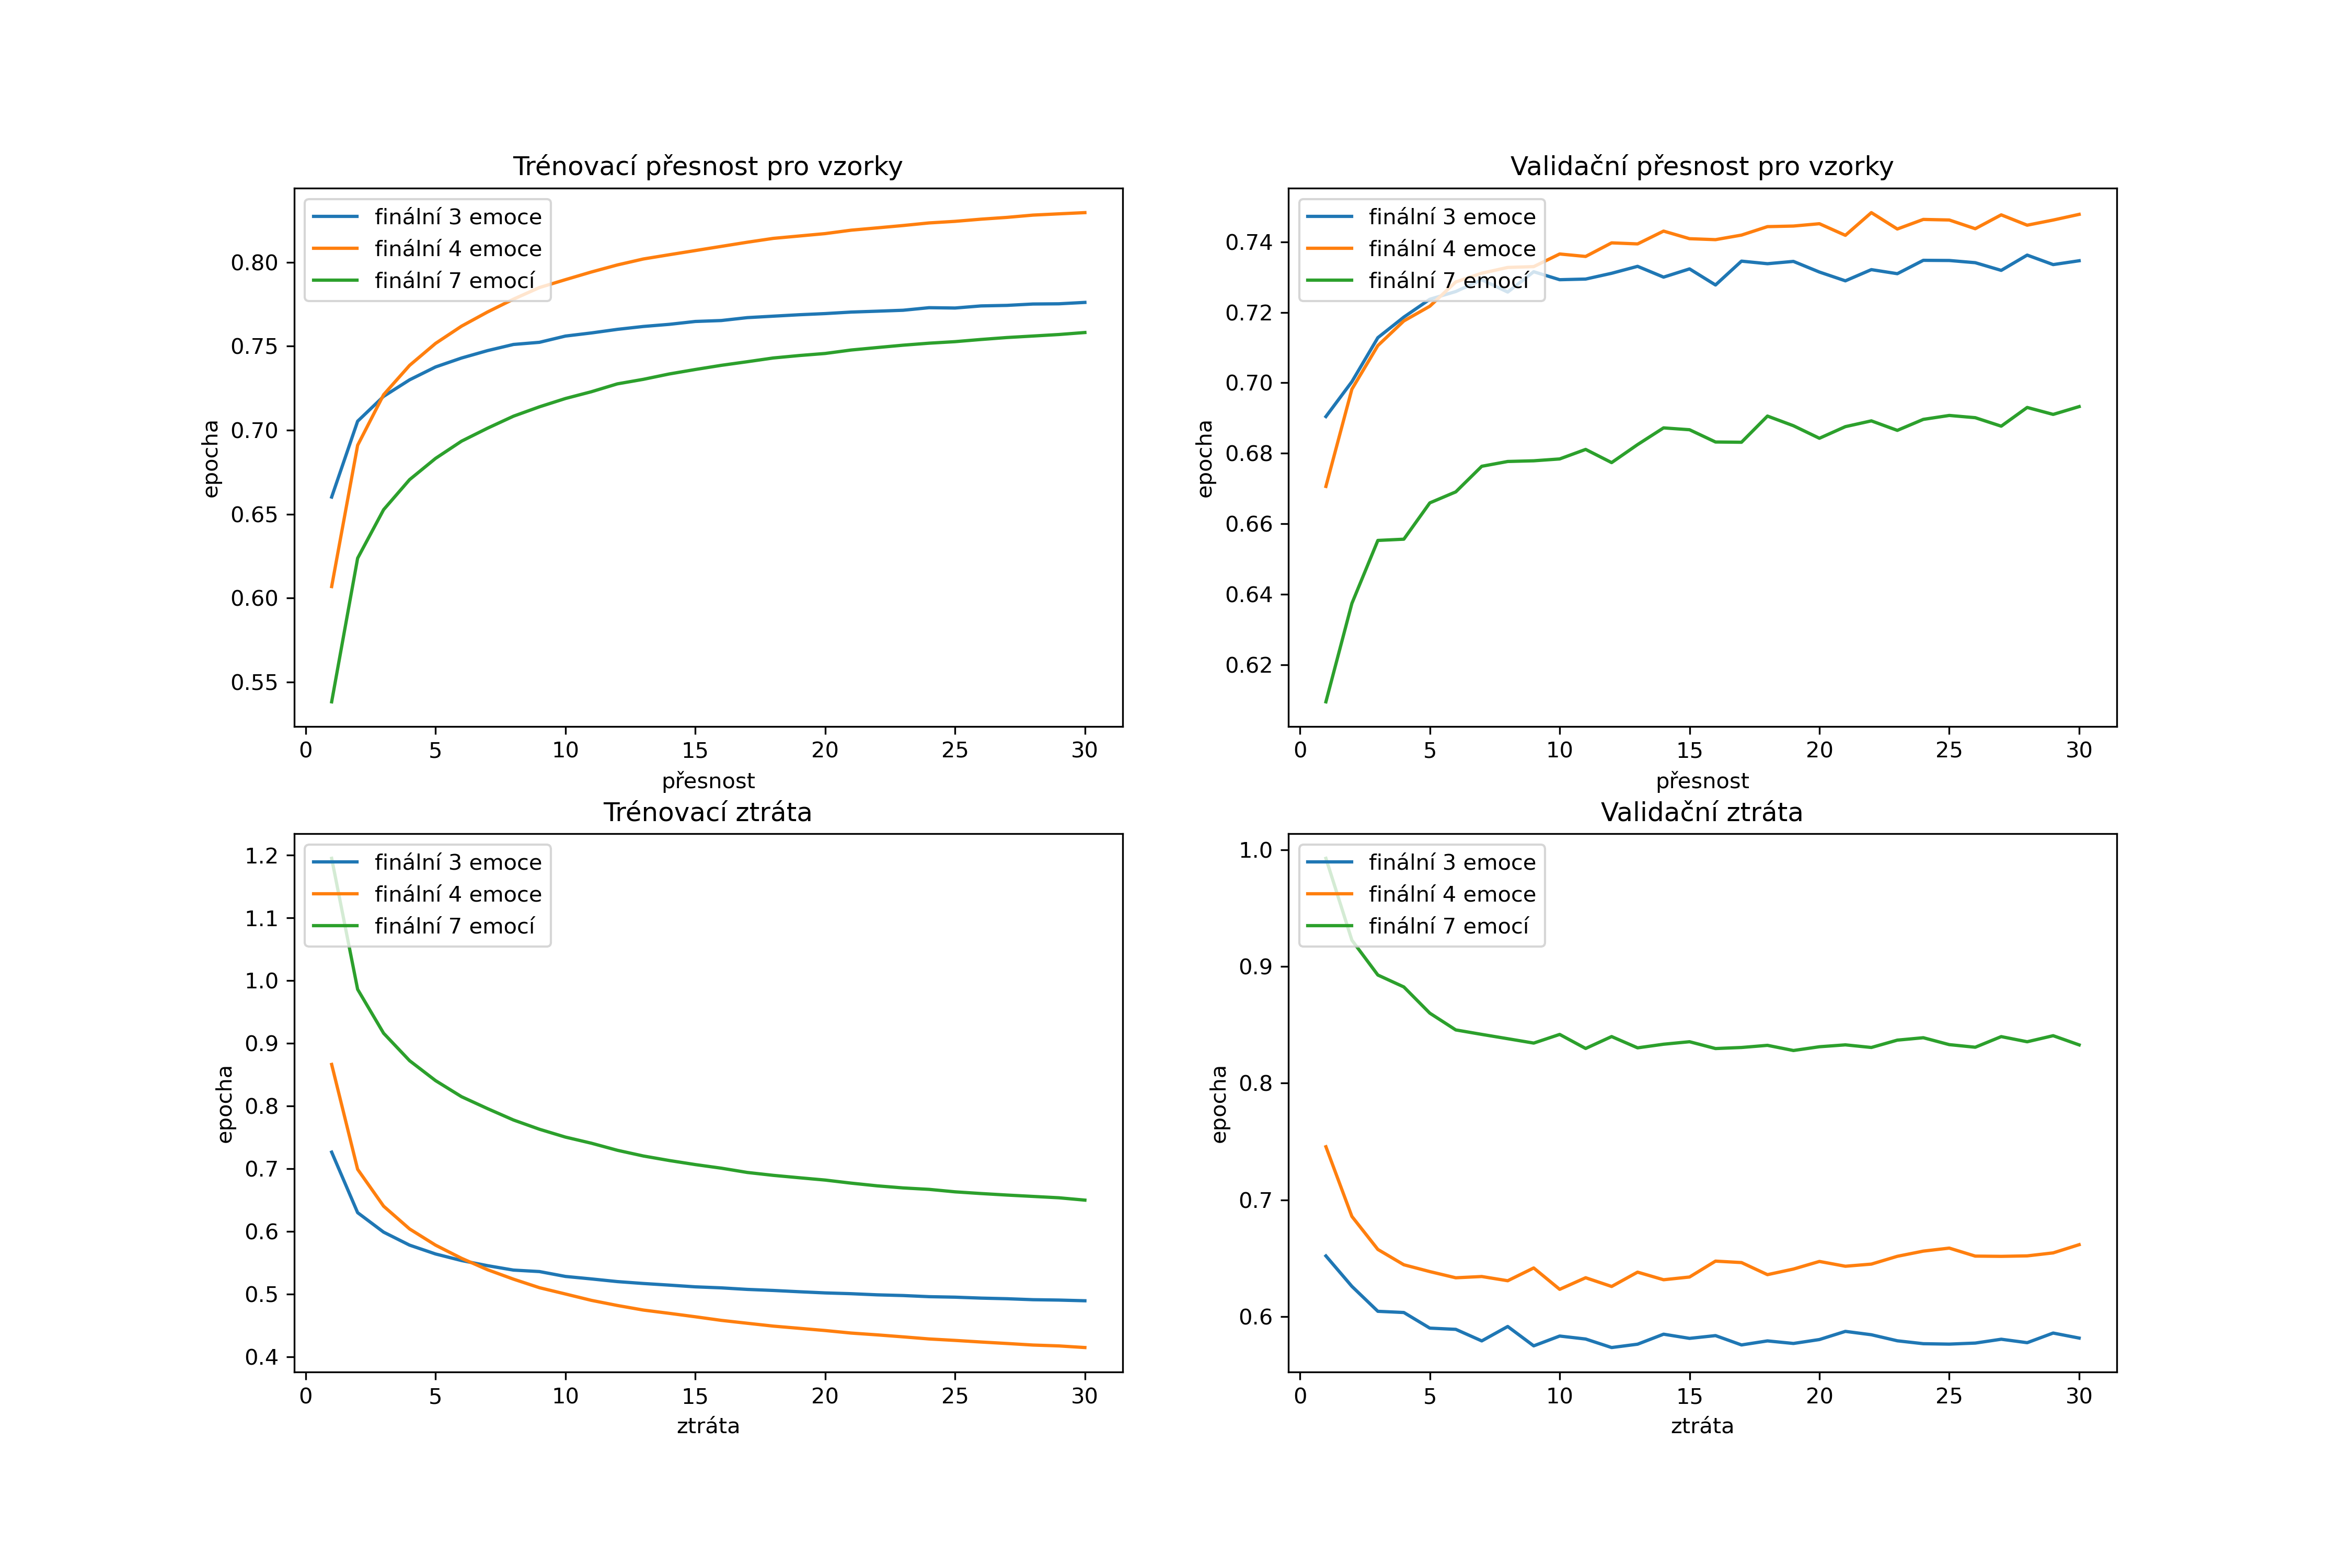
\includegraphics[scale=.5]{training_course-final.png}}
\caption{Přehled průběhu trénování}
\label{fig:final_training_course}
\end{figure}
\FloatBarrier

\chapter{Závěr}

Z volně dostupných datových sad byly vybrány tři anglické datové sady (RAVDESS, SAVEE, TESS) a jedna italská (EMOVO). Byl sjednocen formát nahrávek a byly získány příznaky MFCC. Pro učení modelu byla data z jednotlivých datových sad rovnoměrně rozdělena do trénovací, validační a testovací sady v poměru 80 \%, 10 \% a 10 \%.

V jazyku Python byl vytvořen balíček pro rozpoznávání emocí. Skládal se z modulů pro převod dat, práci s daty, tvorbu klasifikátoru, práci se soubory, tvorbu datových sad, přípravu datových sad a trénování modelu. Balíček především umožňoval snadné vytvoření, uložení a načtení datových sad pro trénování. Zároveň zprostředkovával jednoduché trénování modelu a uložení výsledků trénování pro zpětnou analýzu.

Jako klasifikátor byla zvolena neuronová síť typu MLP. Model byl vytvořen a natrénován pomocí frameworku PyTorch. Prvotně byl vytvořen výchozí model. Následně bylo provedeno a zdokumentováno několik experimentů s cílem vylepšit hyperparametry výchozího modelu. U většiny experimentů měl model tendenci se přeučovat na trénovacích datech, a proto se osvědčilo umístit do skryté vrstvy regularizační vrstvy, které zabraňovaly přeučování.

Na základě proběhlých experimentů byly vytvořeny tři finální modely pro různý počet emocí. Model pro klasifikaci tří emocí dosáhl 75,4 \% přesnosti pro vzorky a 84,7 \% přesnosti pro nahrávky. Při klasifikaci do čtyř tříd dosáhl model na testovací sadě přesnosti pro vzorky 73,6 \% a 92,3 \% přesnosti pro nahrávky. Klasifikátor do sedmi tříd dosáhl na testovací sadě přesnosti pro vzorky 68 \% a přesnosti pro nahrávky 88,5 \%.

Pro zlepšení výsledků klasifikace by nejvíce pomohlo rozšíření datové sady pro trénování. Pomocí regularizačních vrstev lze do jisté míry přeučování modelu zabránit, ale míru přesnosti modelu omezuje nízký počet a různorodost dat. Dalším způsobem, jak vylepšit výsledky klasifikace, je vyzkoušet jiné typy neuronových sítí. V úvahu na příklad přicházejí neuronové sítě typu CNN nebo RNN. V obou případech lze téměř bez změn přidat funkcionalitu do balíčku pro rozpoznávání emocí.

\nocite{*}
\printbibliography[title={Použitá literatura}] % sazba seznamu citací
\addcontentsline{toc}{chapter}{Použitá literatura} % vložení nadpisu do obsahu

\end{document}
